% XeLaTeX can use any Mac OS X font. See the setromanfont command below.
% Input to XeLaTeX is full Unicode, so Unicode characters can be typed directly into the source.

% The next lines tell TeXShop to typeset with xelatex, and to open and save the source with Unicode encoding.

%!TEX TS-program = xelatex
%!TEX encoding = UTF-8 Unicode

\documentclass[11pt]{physics}
\usepackage{amscd}
%\renewcommand{\baselinestretch}{1.15}
\makeatletter
\def\@tocline#1#2#3#4#5#6#7{\relax
  \ifnum #1>\c@tocdepth % then omit
  \else
    \par \addpenalty\@secpenalty\addvspace{#2}%
    \begingroup \hyphenpenalty\@M
    \@ifempty{#4}{%
      \@tempdima\csname r@tocindent\number#1\endcsname\relax
    }{%
      \@tempdima#4\relax
    }%
    \parindent\z@ \leftskip#3\relax \advance\leftskip\@tempdima\relax
    \rightskip\@pnumwidth plus4em \parfillskip-\@pnumwidth
    #5\leavevmode\hskip-\@tempdima #6\nobreak\relax
    \ifnum#1<0\hfill\else\dotfill\fi\hbox to\@pnumwidth{\@tocpagenum{#7}}\par
    \nobreak
    \endgroup
  \fi}
\makeatother
\usepackage[text={6.5in,9in},centering]{geometry}                % See geometry.pdf to learn the layout options. There are lots.
\geometry{a4paper}                   % ... or letterpaper or a5paper or ... 
%\geometry{landscape}                % Activate for for rotated page geometry
%\usepackage[parfill]{parskip}    % Activate to begin paragraphs with an empty line rather than an indent
\usepackage{graphicx}
\usepackage{amssymb}
\newtheorem*{theorem}{\simhei 定理}
\XeTeXlinebreaklocale "zh"
\XeTeXlinebreakskip = 0pt plus 1pt

% Will Robertson's fontspec.sty can be used to simplify font choices.
% To experiment, open /Applications/Font Book to examine the fonts provided on Mac OS X,
% and change "Hoefler Text" to any of these choices.

\usepackage{fontspec,xltxtra,xunicode}
\defaultfontfeatures{Mapping=tex-text}
%\setromanfont[Mapping=tex-text]{Hoefler Text}
%\setsansfont[Scale=MatchLowercase,Mapping=tex-text]{Gill Sans}
%\setmonofont[Scale=MatchLowercase]{Andale Mono}
\newfontfamily{\A}{Times New Roman}
\newfontfamily{\H}{Hei}
\newfontfamily{\K}{Kai}
\newfontfamily{\simsun}[Scale=0.9]{SimSun}
\newfontfamily{\simhei}[Scale=0.9]{SimHei}
\newfontfamily{\fangsong}{FangSong}
\makeindex
\begin{document}
\frontmatter
\title{\K 基础物理课程讲义}
\author{\simhei \small (草稿)}
%\date{}                                           % Activate to display a given date or no date
\maketitle
\tableofcontents
\mainmatter
\chapter{绪论}
\section{物理学与其他自然科学}

   物理学是探讨物质世界的结构和运动基本规律的自然的学科。 
   物质世界存在的形式是多种多样的:实物形式、场的形式。实物形式又按物态可分:固态、液态、气态、等离子态。 
   物质世界是有结构的,结构也是多种多样的:原子有原子结构,分子有分子结构,固体特别是晶体也有明显的结构,我们生存所在的地球也是有结构的。太阳系有太阳系的结构,其核心太阳也是有结构的,而太阳本身也是更大的银河系中极其不起眼的普通一员。银河系中大约$2\times10^{11}$ 个像太阳那样能发光的大大小小的恒星。邻近的若干星系可以组成星系群或星系团。由星系群或星系团可以组成超星系团。(作业:写出$H_2O $分子、地球、太阳系结构)
   
   
   物质世界的运动形式是多种多样的:有宏观的(或经典的)机械运动(或力学运动);有热运动(组成宏观物体的大量宏观粒子的无规则运动);有场的运动,如电磁场的运动(光波就是电磁场运动的一种表现形式);微观粒子有其特有的量子运动。此外物质世界还时时刻刻的发生形形色色的转化。除了物态转化外,还有核反应、化学反应等等。物质的运动和转化都与物质内部存在的相互作用密切有关。研究物质的运动和转化与相互作用的规律是物理学的主要内容。
   
    所以更详细的说,物理学研究物质存在的各种基本形式。它们的性质。运动和转化及内部结构,从而认识这些结构的组元及其相互作用,运动和转化规律的学科。
    
    自然科学是研究自然界各种现象的规律的自然学科,可划分为天文学、力学、物理学、化学、生物学、地质学等。物理学最直接地关心自然界最基本规律。因此牛顿在当时把物理学叫做自然哲学(牛顿划时代的名著名为《自然哲学的数学原理》就反映了这种观念。)物理学成为各个自然科学的基础就不足为奇了。正常物理学的发展和成就应用于天文学 使我们认识了各种天体的本质、认识了星系的形成、认识了行星从诞生到死亡的过程、认识到宇宙演化的历史。产生了诸如天体物理和宇宙学等交叉学科。将物理学的知识应用于化学的研究,是我们认识了化学现象的的机理,从而产生了物理化学、量子化学等交叉学科。而物理理论应用与生命现象的研究则产生了生物物理等交叉学科。
    
    物理学和数学关系怎样?数学的研究对象显然较物理学的抽象,但它也必然是从物质世界中抽象出来的数量或图形的各种关系。(华罗庚:"数学是研究数和形的科学")。物理和数学在其发展过程中是相互促进,共同发展的。最经典的例子是牛顿在奠定经典力学理论的同时创立了微积分的基本理论(牛顿《自然哲学的数学原理》)而爱因斯坦广义相对论适应于近代微分几何,主要是黎曼几何的应用密切相关的。近代物理中规范场理论与数学中的纤维丛理论的关联,以及二十世纪八十年代后用量子场论工具研究拓扑学上的重大课题都是很好的例子。
    
    在学习本课程的过程中,我们可以看到,在许多场合下,借助数学上的一些基本原则往往很容易指示出物理概念。物理规律表现形式发展的来龙去脉,数学工作者在初物理理论是应充分利用自己的长处。但是数学工作者必须熟悉各种各样的物理量,学习各种物理现象的数学描述。
    
    

\section{物理世界的层次}
    学习物理,首先应对我们所面对的物质世界有一个基本的了解。物质世界显然非常复杂,但只要我们能分清层次,也还是能够把握的。  
物理上讨论层次,采用的是数量级分析法(又称为科学计数法),即用$10^n$中的n来比较大小,划分层次。我们面对的物质世界,按其空间尺度大小来分析跨越了42个数量级,即由$10^{-15}\longrightarrow10^{27}$。有人把这个称为物质世界的"四十二个阶段"。空间尺度处于不同数量级的对象往往具有不同的性特点,正因为如此构成了物理学不同分支所研究的对对象。  
人类在日常生活中所接触的对象,虽然大小有别,形态各异(固态、液态、气态或等离子态)但尺寸的量级基本在     左右。这些对象的研究属于宏观物理的范畴。常用的单位是米(m)、分米(dm)、厘米(cm)、毫米(mm)、千米(km)等。  
随着我们对物质结构逐步深入的认识。我们知道物质是由分子组成的,分子则是由原子组成的。原子时有原子核及外围电子组成的。我们研究的对象深入到纳米($nm=10^{-9}$)费米($fm=10^{-15}$)这一尺度范围对象的研究已属于微观物理的范围。另一方面,随着我们的目光转向天空,转向地球之外。我们发现地球不过是太阳系中的一颗行星。讨论行星运动常用的尺度单位是天文单位(AU).一个AU表示日地的平均距离。$$1AU=1.49597892\times10^{11}  \approx1.5\times10^{11}m$$   
太阳系的直径约80个AU,即$10^{13}$的数量级,但是"天外有天"我们引以为豪的太阳不过是银河系中的一个普通的恒星。银河系有近似$2\times10^{11}$颗恒星(它们的质量与太阳质量相近)。讨论银河系的方法常用的尺度单位是光年(ly)或秒差距(pc-parsec)$$1ly=9.460530\times10^{15}m\approx10^{16}$$$$1pc=\frac{1AU}{1”}=\frac{1AU}{\pi/180\times60\times60}=3.085678\times10^{16}m\approx3.26ly$$1pc或1ly与银河系中恒星的平均距离数量级相近。银河系具有盘状结构,银盘直径约$50kpc\sim1.5\times10^{21}$m。
    
         
银河系外有别的星系,数目难以估测。星系也会成固而形成星系团或超星系团。它包括了几千个星系,其尺寸约为1Mpcsim100Mpc。而目前我们所观测的宇宙范围约为$10^{10}pc (10^{26}-10^{27}m)$。下面表格绘出物质世界不同层次对象的物理名称以及研究它们所对应的学科。
         
              粗略地讲,按研究对象的尺度来划分,可将物理学的研究分为微观物理、宏观物理和介观物理。近几十年来,由于微结构技术的发展,制备长度为$\mu m$,线宽为几十个$\mu m$的样品已不太困难,虽然这样的样品包含了$10^8-10^{11}$个原子,但他们在低温下却能显示出电子波的量子干涉现象。这种显现出微观特征的宏观系统称为介观系统,它们是下一代微电子的候选者,把对介观系统的研究通常称为介观物理。
              
\begin{center}
\begin{tabular}{|c|c|c|}\hline  
          对象名称 &  尺度        & 对应的学科 \\ \hline
          粒子     &  $10^{-15}$   & 粒子物理   \\ \hline
          原子核   &  $10^{-14}$   &核物理\\ \hline
          原子     &  $10{-10}$  &原子物理\\ \hline
          分子     &$10^{-9}$    &化学,物理化学\\ \hline
          巨型分子(如DNA)& $\longleftarrow10{-7}\longrightarrow$&介观物理\\ \hline
          及小尺寸样品&$\longleftarrow10\longrightarrow$&生物物理\\ \hline
          宏观物体&$10^7$&固体物理,材料物理,等离子物理\\ \hline
          地球&$10^{13}$&地球物理\\ \hline
          太阳系&$10^{21}$&空间物理\\ \hline
          银河系&$10^{21}$&天体物理\\ \hline
          星系团&$10^{23}$&天体物理\\ \hline
          超星系团&$10^{25}$&天体物理\\ \hline
          可观测宇宙&$10^{26}-10^{27}$&宇宙学\\ \hline
\end{tabular}
\end{center}

(记住n个特征制度:fm,nm,m,AU,pc,$10^{10}pc$)

必须指出,上述物质世界的层次是今日宇宙中的物质世界的层次,而大量观测资料表明宇宙本身是出于变化之中的。按照大爆炸宇宙模型。原始宇宙处于高温,   状态,只有热辐射和     粒子。在宇宙膨胀逐渐冷却的过程中先后形成了原子、分子。以后由于物质密度膨胀加上引力成固效应,产生星系,星系团,同时   物质和恒星产生各种各样的物质形态逐渐呈现出当今物质世界的各个层次。
\section{物质的基本组成,基本相互作用。“标准模型”}  
物理学的理论可以分为唯象理论和基础理论两大范畴,这两方面理论是相互补充、相互促进的。而物理学最前沿的领域是研究物质世界的基本组成和基本相互作用的基础理论。物质世界的一切现象追根寻源,都应该用物质的基本组成的及它们之间基本相互作用规律来解释。  
十九世纪末二十世纪初,物理界所谓的“基本粒子”是:

分子-原子 
\[\left<   \begin{array} {l}  \mbox{电子}\\
 {\mbox{原子核}\left< \begin{array}{c} \mbox{质子}\\ \mbox{中子} \\  
 \end{array}  \right.} 
 \end{array}   \right.  \]
以及传递电磁相互作用的光子    
以后陆续发现了上述粒子的反粒子
    
正电子(电子的反粒子,1932)   
反质子(1956)    
从二十世纪三十年代到六十年代发现了越来越多的"基本粒子". 三超子,中微子,反中微子等等。  
“基本粒子”家属的成员越来越多,从几十种发展到几百种。物理学家开始怀疑这些粒子是否都能成为“基本粒子”呢?从二十世纪六十年代开始物理学家通过研究这些粒子的分类以及它们的对称性中,逐渐认识到之中大多数是由更基本的粒子组成的。陆陆续续地提出了一些模型,经过反复推敲,又经过各种物理实验和其他观测的旁证的筛选,在二十世纪七八十年代,逐渐形成了粒子物理的“标准模型”,并为大多数粒子物理专家所接受。

\subsection{粒子物质“标准模型"}
\begin{enumerate}
\item
最基础的粒子包括自旋为$\frac{\hbar}{Z}$的弗末子和自旋为$\hbar$的整数倍($0\hbar,\hbar,2\hbar$)的玻璃粒子两大类。
 
   弗末子有三代,每一代包括六和夸克和两种粒子,没一种弗末子都有其反粒子,因此总共有48种弗末子。
   
$
\left\{  \begin{array}{llll}  
\mbox{夸克}  &  {\left(\begin{array}{ccc}  u^1  &  u^2  &  u^3 \\ d^1 & d^2  & d^3 \\ \end{array}  \right)}  &   { \left(  \begin{array}{ccc}   c^1  &  c^2   &  c^3  \\ s^1  &  s^2  & s^3 \\  \end{array}  \right) }  &  { \left( \begin{array} {ccc}  t^1  &  t^2  &  t^3  \\ b^1  &  b^2  &  b^3 \\  \end{array}  \right) }\\
 \mbox{轻子}  &   { \left ( \begin{array}{c}  \nu_e\\ e \\  \end{array}  \right) }    &  {\left (\begin{array}{c}\nu_\mu\\\mu\\ \end{array} \right) }  &  { \left( \begin{array}{c} \nu_\tau \\ \tau \\  \end{array}  \right) } \\
\end{array}  \right.$

  
 其中c夸克,b夸克,t夸克(严格说是包括这三种夸克的       )发现较晚,分别是在1974年、1977年1996年就被发现的。其中美籍华裔物理学家因为发现了c夸克而获得了1976年度诺贝尔物理奖。  
\item
自旋为$\hbar$的玻璃子又称为规范玻璃子,它们是传递相互作用的粒子(它们也可能有自相互作用。)由规范玻璃子传递的相互作用包括有强相互作用、弱相互作用、电磁相互作用。这些相互作用、具有一定的规范对称性,顾又称规范相互作用。标准模型提出的规范对称性用$SU(3)_c \times SU(2)_L \times U(1)_Yf $群来表示。这个直乘群有十二个生成元,固有十二种规范玻璃色子。
  
 规范玻色子 $\left< \begin{array}{l} g^i(i=1,2.....8)\\ w^+                     \\  \end{array}  \right. $   
\item 
描述弱相互作用、电磁相互作用的规范对称性实际上是破缺的,为了实现对称性的自发破缺,在理论上又引入了自旋为$0\hbar$的数学粒子(H),通常称为Higgs粒子。  
\item 有一种观点认为引力相互作用是由自旋为2$\hbar$的引力子(G)传递的。  
\item 标准型中包含了48+12+1+1=62种基本粒子会不会这些粒子可以用更基本的对象来说呢?目前这仍然是一个谜团,所谓弦理论、起弦理论的提出与这个谜团有一定关系。  
\end{enumerate}
 \subsection{四种基本相互作用  }
 粒子之间的相互作用包括强相互作用,弱相互作用,电磁相互作用。  
下面的表格指明了各种基本相互作用的传递者,它们的质量,这些相互作用的力程,作用强度(通常以质子作为代表比较四种相互作用和作用强度,因为质子是一种可以同时参与四种相互作用的粒子,去两个质子相距r=2.5fm时,比较四种相互作用的强度,表现了相互作用强度数量级上有明显的差别。)

\begin{center}
 \begin{tabular}{|c|c|c|c|c|}\hline
相互作用类型  &  强  &  电磁&  弱& 引力 \\ \hline
作用传递者   & $ g^i $ & $\gamma $ & $ W^\pm Z $& G  \\   \hline
质量(Ger)  &  0  & 0 &  80.2  91.2 & 0  \\ \hline  
力程(fm)   & 1.413  & $ \infty $ &  0.00246  & $ \infty $  \\ \hline
作用强度     &0.15  & 0.0073  & $ 6.34\times10^{-4} $ &  $5.9\times10^{-39}$ \\  \hline
宏观表象     &无  &  有  &  无&有\\  \hline  
\end{tabular}
\end{center}
  
(*  细结构常数 
$ \alpha=\frac{e^2 }{4 \pi \hbar c } \approx \frac{1}{371}\approx 0.0073$  )    
 \[\frac{e^2}{4 \pi \varepsilon_0}=1.44ev.nm \]
 \[hc=1.24\times10^3ev.nm\]
 \[\alpha=\frac{e^2}{4 \pi \varepsilon_0\hbar c=0.0073}\]
\section{物理学及其单位制,量纲}
  
 物理现象的定量描述要用物理量,物理规律用不同物理量之间的关系(方程式)来表示,物理量的数值取决于所选取的单位。  
 \subsection{单位制 }
\subsubsection{基本量和导出量;基本单位和导出单位}
物理量之间由定义和定理互相联系,可以选择少数几个物理量,规定其单位。这些物理量称为基本量,它们的单位称为基本单位。而其它物理量则由定义或物理定律导出其单位。这些量称为导出量,相应的单位称为带出单位。  
\subsubsection{单位制}  选定那些物理量为基本量,规定其单位,其它物理量有定义或物理定律导出其单位。这一规定称为    一种单位制。  
物理学中常用的单位有国际单位制(SI),高斯单位制,自然单位制。
  
\subsubsection{国际单位制(SI)基本量,基本单位  }

\begin{center}
\begin{tabular}{|c|c|}\hline
基本量     &     基本单位  \\ \hline
长度  l  &          米(m)  \\ \hline
时间 t   &        秒(s)    \\  \hline
质量m  &           千克(Kg) \\  \hline
电流强度i   &      安培(A)  \\  \hline
温度T    &          开尔文(K)  \\  \hline
发光强度I    &      坎德拉(cd) \\   \hline
物质的量 n    &     摩尔(md)  \\    \hline
\end{tabular}
\end{center}
  
关于基本量的基本单位的规定随着物理学的发展有所变迁。  
 $ 1mol=6.0221367\times10^{23}$(阿伏伽德罗常数)    
 发光强度的定义为$I=\frac{\Phi}{\Omega}  $   其中 $\Phi$为光通量。它是光能通量与视觉函数的乘积。$\Omega$为主体角。描述可见光的强弱与人的视觉有一定关系。   
 物理学的各个分支为了讨论方便,也规定了一些导出量的单位。如力学中的N,W,Pa.电磁学中的C(库伦)F(法拉)H(亨利)等这些单位的含义应有其与其它物理量,特别是基本量的关系来确定。
  
\subsection{量纲及量纲分析   }
\subsubsection{量纲,量纲指数,量纲法则}
以理学为例,在力学中有三个基本单位:长度、质量、时间.分别用L、M、T表示这三个基本量,任一物理量(A)就其单位量度来说,总可以表示为这三个量的乘方之积。$$ [A]=L^\alpha M^\beta T^\gamma$$ 例$[v]=LT^{-1}$,  $[F]=LMT^{-2}$    
上述表达式称为力学量A的量纲式,等式右边称为A的量纲。$\alpha$,$\beta$,$ \gamma $ 称为量纲指数。  
量纲法则:只有量纲相同的物理量才能相加,相减或相等。

\subsubsection{量纲分析}
 利用量纲概念以及量纲法则有关     作定向分析,称为量纲分析。  
 用量纲分析可以处理以下一些问题:
\begin{enumerate}
\item 单位换算:单位制之间进行换算。例:$1N=10^5dy$   

\item 验证公式  

\item 为推到复杂公式提供线索。  
例:直升飞机  在空中消耗的功率为P。仅取决于机翼长为l,飞机机身重G和空气密度$\rho$,三个因素。若机身重量增加一倍。直升飞机消耗功率增大为原来的几倍?$$\dim P=(\dim l)^\alpha (\dim G)^\beta (\dim \rho)^\gamma$$   $\dim P=ML^2T^{-3}$,  $\dim l=L$  ,  $\dim G=M L T^{-2}$  ,  $\dim \rho =ML^{-3}$    
可得:  $\alpha=-1$ , $\beta=\frac{3}{2}$  ,  $\gamma=-\frac{1}{2}$     
 当G增大一倍时,P应增大为原来的$2^\frac{3}{2}$倍。

\item 有系统的固有参数,分析系统的特征物理量
  
 例:质量为m的一物体在空气中由高处自由下落,设空气阻力与物体速度成正比\[ \overrightarrow{F}=-\alpha\overrightarrow{v}  \text{($\alpha$与物体形状有关)  }  \]
 解:以开始下落处为坐标原点,竖直向下方向为X轴正方向。则运动方程为:$$m \frac{d^{2}x}{dt^{2}}=-\alpha \frac{dx}{dt}+mg$$    
其解为:$x=(\frac{m}{\alpha})^2 g (e^{-\frac{\alpha}{m}t}-1)+ \frac{m}{\alpha}gt$
  
  从量纲分析看,其固有参数的量纲式为:$$[m]=M^1$$  $$[\alpha]=[\frac{F}{v}]=M^1T^{-1}$$   $$[g]=L^1T^{-2}$$  
  
  显然有:$$[\frac{m}{\alpha}]=T$$   $$[\frac{m}{\alpha}g]=L^1T^{-1}$$  $$[(\frac{m}{\alpha})^2g]=L$$ 
  
  若将:$\frac{m}{\alpha}\equiv \tau$  , $\frac{m}{\alpha}g \equiv v_c$  ,  $(\frac{m}{\alpha})^2g \equiv L_c $ 
  
  其解可表示为:$$x=L_c(e^{-\frac{t}{c}}-1)+ v_ct $$   
不难由上式看出:$\tau$,$v_e$ 以及$L_c$的物理含义,特别是:$v=v_c(1-e^{-\frac{t}{\tau}})$
  
 又如简谐振子,其系统的固有参数为:m,k。方程为:$m \frac{d^{2}x}{dt^{2}}=kx=0d$  $$[m]=M$$  $$[K]=[\frac{F}{x}]=MT^{-2}$$  方程的解为: $x=Acos(\omega t+\varphi_0)$ 
  
  而$[\sqrt{\frac{k}{m}}]\equiv \omega$ 正是系统的固有频率(特征频率)。
  
   
\item 对物理结果进行量纲分析判断其大概形式如在空气中以初速度$v_0$上抛。(参量为m,g,$\alpha$,$v_0$) 

可以判断其上抛高度为:$$H=\frac{v_0^2}{g} f ( \frac{\alpha v_0}{mg})$$ 注意到:$\frac{\alpha v_0}{mg}$无量纲.
\end{enumerate}




\chapter{力学与相对论}
正如绪论中所介绍的,力学(经典力学)研究的对象是物体的机械运动,更准确得说是研究若引力场中宏观物体的低速运动。
\begin{center}
\begin{align}
\text{\simhei{研究对象}:}& \text{\underline{宏观物体}在\underline{弱引力场}中\underline{低速运动}}  \notag \\
&\text{($\frac{GM}{rc^2}\ll1$时称为弱引力场,时空平直)} \notag \\
&\text{($\frac{v}{c}\ll1$时称为低速运动,伽利略、牛顿时空)}\notag \\
&\text{($\frac{H}{\bar{h}}\gg1$时称为宏观物体,物体运动状态可以用经典力学描述)}\notag
\end{align}
\end{center}

$H$为体系具有作用量的纲的“自然”动力学变量。前两个条件不满足我们必须用相对论(狭义相对论、广义相对论)来讨论,后一个条件不满足必须用量子力学来讨论。

我们将从最简单的质点讨论起,然后讨论质点为固体和流体等较为复杂的情况。

经典力学的内容包括运动学和动力学两个方面,运动学研究物体运动状态如何描述,以及描述运动状态的物理量之间的关系。而动力学研究物体运动状态的变化和物体与外界相互作用的关系。通常所说的力学规律之的主要是动力学规律。

力学规律的表述有几种不同的形式,用数学的语言来讨论,分别是:
\[
\begin{cases}
\text{不变分形式——牛顿形式(微分形式,积分形式)}\\
\text{变分形式(\A{variational form})}
	\begin{cases}
	\text{微分形式}\begin{cases}
		\text{拉格朗日力学(\A{Lagrangian mechanics})}\\
		\text{哈密顿力学(\A{Hamiltonian mechanics})}
		\end{cases}\\
	\text{积分形式——最小作用量原理(\A{Principle of least action})}
	\end{cases}
\end{cases}
\]

通常把力学规律的变分形式成为分析力学。分析力学的形式可以推广到物理学的其他领域,因而有着更普遍的意义。

本课程主要介绍牛顿形式、分析力学部分只做简略的介绍。

\section{质点运动的描述}
\subsection{质点、参考系、坐标系}
在物理学中为了研究方便,通常将研究的对象“理想化”,突出主要特征,忽略其次要因素,从而简化相应的物理模型以及相应的数学模型。力学中所谓的质点、刚体(有限自由度)、理想流体,完全弹性介质(以上为无线自由度)。热力学和统计物理学中所谓理想气体,电磁学中所谓点电荷、偶极子,理想导体都属于这样的模型。

以质点为例。

\subsubsection{质点}若我们考察的物体在所研究的问题中物体本身的大小和形状比之所考察的运动的线度小得多时,我们可以突出物体所具有的质量在所在空间中占有一定位置,这样两个因素用$(m,\vec{\gamma})$来描述,而忽略形状、大小和内部运动等次要因素。把物体视为具有质量而没有大小的对象。这就是所谓“质点”的概念。例如:当我们讨论地球绕太阳的公转运动时,我们把地球视为质点。而讨论地面上不同纬度处不同物体运动的差别时,我们必须把地球当作一个绕固定轴转动的刚体了。

要描述质点的运动首先要建立参考系、坐标系。
\subsubsection{参照系}

参照系的问题实际上是不同的观测者的问题。
\begin{description}
\item[参照空间]与参照物固连的三维空间;
\item[参照时间]与参照物固连的时钟所记录的时间;
\end{description}
参照空间与之固连的时钟组合称为参照系,通常用$S(O-XYZ),S'(O'-X'Y'Z')$来表示。在相对论的情况下,参照系表示为$S(O-ct,XYZ),S'(O'-ct',X'Y'Z')$。
\subsubsection{坐标系}
为定量地描述质点在参照系中的位置,而在参照空间中选定一组基矢(通常是正交的)以及相应的一组坐标,这样就可以用数学来表述空间中的矢量了。

对于三维的平直空间,常用的坐标系有:
\begin{description}
\item[直角坐标系]基矢为$(\vec{e_x},\vec{e_y},\vec{e_z})$或$(\vec{e_i},\vec{e_j},\vec{e_k})$,坐标记为$(x,y,z)$;
\item[平面极坐标]基矢为$(\vec{e_r},\vec{e_\varphi})$,$\vec{e_r},\vec{e_\varphi}$分别沿着$r,\varphi$增加的方向,随质点位置而变;
\item[球坐标系]基矢为$(\vec{e_r},\vec{e_\theta},\vec{e_\varphi})$,分别表示径、经度、纬度;
\item[柱坐标系]基矢为$(\vec{e_k},\vec{e_\varphi},\vec{e_z})$,对研究有对称的问题较方便;
\end{description}

\begin{figure} [ht]
\centering
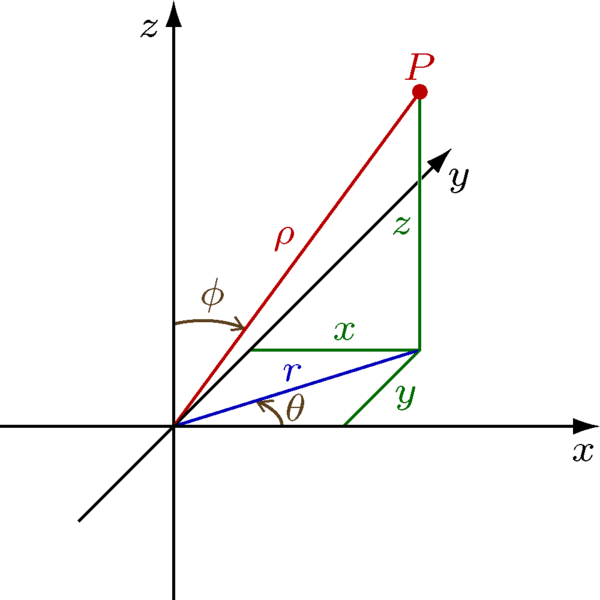
\includegraphics[scale=.35]{600px-Spherical_Coordinates.png}
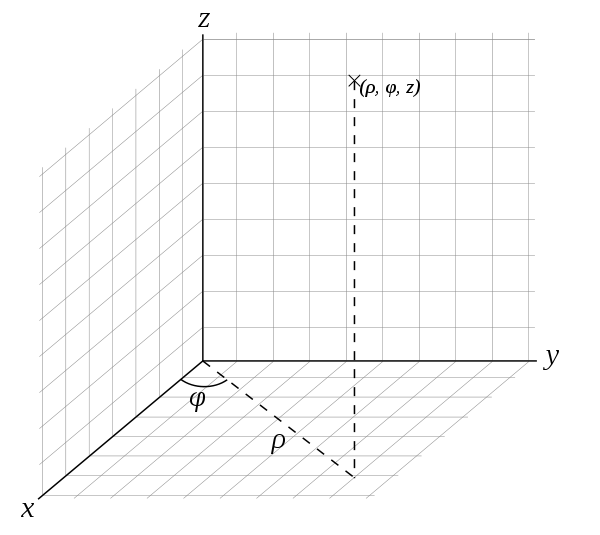
\includegraphics[scale=.4]{600px-Cylindrical_with_grid.svg.png}
\caption{\simsun 用球坐标系(左)和柱坐标系(右)表示三维空间内一个点的位置}
\label{600px-Cylindrical_with_grid.svg.png_600px-Spherical_Coordinates.png}
\end{figure}

此外还有一种自然坐标系(或本性坐标系),这是一种质点瞬时运动状态决定基矢的坐标系。其基矢为$\vec{e_\iota},\vec{e_n},\vec{e_\nu}$(或$\vec{c},\vec{n},\vec{b}$)分别表示该时钟质点运动的切向、主法向和次法向。

\subsection{质点运动的描述}
经典力学史研究物体的机械运动,所谓机械运动是物体空间位置随时间变动而变动的,物体在空间的位置要用矢量来描述,运动则用位置对事件变量$t$的依赖关系以及对时间的一次微商(速度),二次微商(加速度)等物理量来描述,因此要熟悉机械运动的描述,必须有关矢量和矢量的微分、积分运动。

我们还是首先将注意力集中在质点运动的描述上。

\subsubsection{位置矢量$\vec{\gamma}$}
$\vec{\gamma}$在各坐标系下的表示:\begin{description}
\item[直角坐标系]
	$\vec{\gamma}=x\vec{i}+y\vec{j}+z\vec{k}$,
	$\vec{\gamma}=(x,y,z)$
\item[极坐标系]
	$\vec{\gamma}=r\vec{e_r}$,$\vec{e_r}$再由$\varphi$决定,
	$\vec{\gamma}=(r,\varphi)$
\item[球坐标系]
	$\vec{\gamma}=r\vec{e_r}$,$\vec{e_r}$再由$\theta,\varphi$决定,
	$\vec{\gamma}=(r,\theta,\varphi)$
\item[柱坐标系]
	$\vec{\gamma}=\rho\vec{e_\rho}+z\vec{e_z}$,
	$\vec{e_\rho}$再由$\varphi$决定,
	$\vec{\gamma}=(\rho,\varphi,z)$
\end{description}


\subsubsection{速度矢量$\vec{v}$}\begin{description}
\item[定义(一维运动)]
$\vec{v}=\lim_{\varDelta t\to0}\frac{\varDelta x}{\varDelta t}=\frac{dx}{dt}$
\item[定义(三维空间)]
$\vec{v}=\frac{d\vec{r}}{t}=\lim_{\varDelta t\to0}\frac{\varDelta\vec{r}}{\varDelta t}$
\item[在直角坐标系下以分量表示]

\begin{align}
\vec{v}&=\frac{d\vec{r}}{t}=\frac{d}{dt}(x\vec{i}+y\vec{j}+z\vec{k}) \notag \\
&=\frac{dx}{dt}\vec{i}+x\frac{d\vec{i}}{dt}+\frac{dy}{dt}\vec{j}+y\frac{d\vec{j}}{dt}+\frac{dz}{dt}\vec{k}+z\frac{d\vec{k}}{dt} \notag \\
&=\frac{dx}{dt}\vec{i}+0+\frac{dy}{dt}\vec{j}+0+\frac{dz}{dt}\vec{k}+0=\dot{x}\vec{i}+\dot{y}\vec{j}+\dot{z}\vec{k} \notag
\end{align}

\item[在平面极坐标系下以分量表示]
\begin{align}
\vec{v} &= \frac{d\vec{\gamma}}{dt} = \frac{d}{dt}(r\vec{e_r}) =\frac{dr}{dt}\vec{e_r}+r\frac{d\vec{e_r}}{dt} \notag \\
&=\dot{r}\vec{e_r}+r\dot{\varphi}\vec{e_\varphi} =v_r\vec{e_r}+v_\varphi\vec{e_\varphi} \notag
\end{align}
\[\text{注意到其中}\frac{d\vec{e_r}}{dt} = \frac{d}{dt} (\cos\varphi \vec{i}+\sin\varphi\vec{j})=(-\vec{i}\sin\varphi+\vec{j}\cos\varphi)\frac{d\varphi}{dt} = \dot{\varphi}\vec{e_\varphi}\]
$v_r,v_\varphi$分别称作径向速度与切向速度。
\item[在球坐标系下以分量表示]
$\vec{v} = \dot{r} \vec{e_r} + r\,\dot\theta\,\vec{e_\theta} + r\,\dot\varphi\,\sin\theta \vec{e_\varphi} $
\end{description}

\subsubsection{加速度矢量$\vec{a}$}\begin{description}
\item[定义]$\vec{a}=\frac{d\vec{v}}{dt}$
\item[在直角坐标系下以分量表示]$\vec{a}=\ddot{x}\vec{i}+\ddot{y}\vec{j}+\ddot{z}\vec{k}$
\item[在平面极坐标系下以分量表示]
\begin{align}
\vec{a} &= \frac{d\vec{v}}{dt} =\frac{d(\dot{r}\vec{e_r}+r\dot{\varphi}\vec{e_\varphi})}{dt} =\ddot{r}\vec{e_r}+\dot{r}\frac{d\vec{e_r}}{dt}+\dot{r}\dot{\varphi}\vec{e_\varphi}+r\ddot{\varphi}\vec{e_\varphi}+r\dot{\varphi}\frac{d\vec{e_\varphi}}{dt} \notag \\
&=(\ddot{r}-\dot{r}\dot{\varphi}^2) \vec{e_r}+(2\dot{r}\dot{\varphi}+r\ddot{\varphi})\vec{e_\varphi} = a_r\vec{e_r}+a_\varphi\vec{e_\varphi} \notag
\end{align}
\[\text{注意到其中}\frac{d\vec{e_\varphi}}{dt} = \frac{d}{dt} (-\vec{i}\sin\varphi+\vec{j}\cos\varphi) = (-\vec{i}\cos\varphi-\vec{j}\sin\varphi)\frac{d\varphi}{dt}=-\dot\varphi\vec{e_r}\]
$a_r,a_\varphi$分别称作径向加速度与切向加速度。
\item[在球坐标系下以分量表示]
\begin{align}
\vec{a} = & \left( \ddot{r} - r\,\dot\theta^2 - r\,\dot\varphi^2\sin^2\theta \right)\vec{e_r} \notag \\
&+\left( r\,\ddot\theta + 2\dot{r}\,\dot\theta - r\,\dot\varphi^2\sin\theta\cos\theta \right) \vec{e_\theta} \notag \\
&+\left( r\ddot\varphi\,\sin\theta + 2\dot{r}\,\dot\varphi\,\sin\theta + 2 r\,\dot\theta\,\dot\varphi\,\cos\theta \right) \vec{e_\varphi}   \notag
\end{align}
\end{description}

\subsubsection{角速度矢量$\vec{\omega}$}
质点绕某一点转动时,常引入角速度矢量,常定义为$\vec{\omega}=\omega\vec{k}$,其中大小$\omega=\frac{d\varphi}{dt}$,方向$\vec{k}$由转轴方向的右手螺旋法则确定。

\begin{figure} [ht]
\centering

\includegraphics[scale=.35]{352px-Angular_velocity.svg.png}
\caption{$\vec{v}=\vec{\omega}\times\vec{r}$}
\label{352px-Angular_velocity.svg.png}
\end{figure}

后面我们可以看到刚体的运动可以分解为任意代表点的平动和绕该点的一个转动,因此描述刚体的运动常用到角速度矢量。

\section{参照系变换}
同一个物体的运动,在不同的参照系中观测,相应的运动学描述是不同的,但既然是同一物体的运动,不同参照系对他运动状态的描述——$\vec{r},\vec{v},\vec{a}$或$\vec{r}',\vec{v}',\vec{a}'$之间——是应该有联系的。了解他们之间的关系,对于分析许多现象是有帮助的。

例如我们常常需要比较:
\begin{center}
\begin{align}
\text{\simhei{例}:}& \text{地面参照系与地心参照系}  \notag \\
&\text{地球参照系与太阳参照系}\notag \\
&\text{实验室参照系与质心参照系} \notag
\end{align}
\end{center}



为叙述方便,在比较两个参照系时,指定某一参照系为静参照系(记作$S(O-XYZ)$),而另一个参照系为动参照系(记作$S'(O'-X'Y'Z')$)。在$S$系中观测到的运动指的是$(\vec{v},\vec{a})$称为\underline{绝对运动},而由$S'$系中观测到的运动称为\underline{相对运动},由$S'$相对于$S$运动而引起的\underline{附加速度$\vec{v_c}$}、\underline{附加加速度$\vec{a_c}$}称为牵连速度。应该指出,这里所谓的“静”与“动”,所谓“绝对”与“相对”,这些概念本来就不是绝对的,而是相对的。

必须指出,在经典力学中,认为不同参照系的时钟是相同的($t=t'$),即不同观测者所携带的时钟记录的时间是相对的($\varDelta t = \varDelta t'$),这是我们假设弱引力、低速运动的结果。

(相对论情况下为$S(O-tXYZ),S'(O'-X'Y'Z')$)
\subsection{$S'$系相对于$S$系作匀速直线运动}
\begin{align}
&\because \vec{\varDelta r} = \vec{\varDelta r'}+\vec{\varDelta R},\varDelta t = \varDelta t' \notag \\
&\therefore \frac{\vec{\varDelta r}}{\varDelta t} =\frac{\vec{\varDelta r'}}{\varDelta t}+\frac{\vec{\varDelta R}}{\varDelta t} \notag  \\
&\therefore \vec{v} =\vec{v'}+\vec{u} \notag
\end{align}
\begin{figure} [ht]
\centering
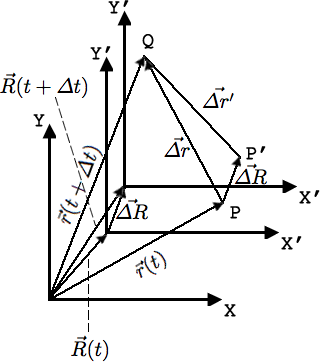
\includegraphics[scale=0.5]{frame_transform1.png}
\caption{\simsun 在$S$系中观测到的运动是从$P$到$Q$,在在$S'$系中观测到的运动则是从$P'$到$Q$}
\label{frame_transform1.png}
\end{figure}
\[ \frac{d\vec{u}}{dt}=0 \Rightarrow \vec{a}=\vec{a'} \]
\[
\text{结论:若$S'$相对$S$作匀速直线运动}
\begin{cases}
\vec{v}=\vec{v'}+\vec{u}\\
\vec{a}=\vec{a'}\\
\end{cases}
\]

\subsection{$S'$系相对于$S$系作任意方式平动}
设$\frac{d\vec{R}}{dt}=\vec{u},\frac{d\vec{u}}{t}=\vec{w}$,则类似地可得:
\[ \vec{v}=\vec{v'}+\vec{u}\quad \vec{a}=\vec{a'}+\vec{w}\]
\subsection{$S'$系相对于$S$系作匀角速度转动}
\begin{align}
&\because \vec{\varDelta r} = \vec{\varDelta r'}+\vec{\varDelta r_f},\varDelta t = \varDelta t' \notag \\
&\therefore \frac{\vec{\varDelta r}}{\varDelta t} =\frac{\vec{\varDelta r'}}{\varDelta t}+\frac{\vec{\varDelta r_f}}{\varDelta t} \notag  \\
&\therefore \vec{v} =\vec{v'}+\vec{\omega}\times\vec{r'} \notag
\end{align}

\begin{figure} [ht]
\centering
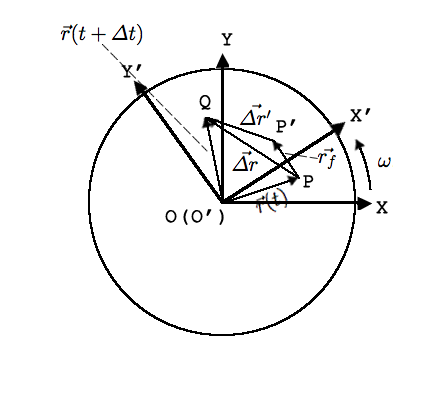
\includegraphics[scale=0.5]{frame_transform2.png}
\caption{\simsun 在$S$系中观测到的运动是从$P$到$Q$,在在$S'$系中观测到的运动则是从$P'$到$Q$}
\label{frame_transform2.png}
\end{figure}
\[\vec{a}=\frac{d\vec{v}}{dt}=\frac{d(\vec{v'}+\vec{\omega}\times\vec{r'})}{dt}=\frac{d\vec{v'}}{dt}+\frac{d(\vec{\omega}\times\vec{r'})}{dt}\]
\[\frac{d\vec{v'}}{dt}=\frac{d(\dot{x}\vec{i'}+\dot{y}\vec{j'}+\dot{z}\vec{k'})}{dt}=\ddot{x}\vec{i'}+\dot{x}\frac{d\vec{i'}}{dt}+\ddot{y}\vec{j'}+\dot{y}\frac{d\vec{j'}}{dt}+\ddot{z}\vec{k'}+\dot{z}\frac{d\vec{k'}}{dt}\]
\begin{align}
&\because \frac{d\vec{i'}}{dt}=\vec{\omega}\times\vec{i'},\ \frac{d\vec{j'}}{dt}=\vec{\omega}\times\vec{j'},\ \frac{d\vec{k'}}{dt}=\vec{\omega}\times\vec{k'} \notag \\
&\therefore \dot{x}\frac{d\vec{i'}}{dt}+\dot{y}\frac{d\vec{j'}}{dt}+\dot{z}\frac{d\vec{k'}}{dt} = \vec{\omega}\times(\dot{x}\vec{i'}+\dot{y}\vec{j'}+\dot{z}\vec{k'})= \vec{\omega}\times\vec{v'}\notag \\
&\therefore \frac{d\vec{v'}}{dt}=\vec{a'}+\vec{\omega}\times\vec{v'}\notag
\end{align}
\begin{align}
\frac{d(\vec{\omega}\times\vec{r'})}{dt} &= \vec{\omega}\times\frac{d\vec{r'}}{dt}=\vec{\omega}\times\frac{d(r_x\vec{i'}+r_y\vec{j'}+r_z\vec{k'})}{dt} \notag \\
&= \vec{\omega}\times(\dot{r_x}\vec{i'}+r_x\frac{d\vec{i'}}{dt}+\dot{r_y}\vec{j'}+r_y\frac{d\vec{j'}}{dt}+\dot{r_z}\vec{k'}+r_z\frac{d\vec{k'}}{dt}) \notag \\
&=  \vec{\omega}\times(\vec{v'}+r_x\omega\times\vec{i'}+r_y\omega\times\vec{j'}+r_z\omega\times\vec{k'}) \notag \\
&=  \vec{\omega}\times(\vec{v'}+\omega\times\vec{r'}) \notag \\
&=  \vec{\omega}\times\vec{v'}+ \vec{\omega}\times\vec{\omega}\times\vec{r'}\notag
\end{align}
\[
\therefore\vec{a}=\vec{a'}+\vec{\omega}\times(\vec{\omega}\times\vec{r'})+2\vec{\omega}\times\vec{v'} = \vec{a'} + \vec{a_l} + \vec{a_{col}}
\]
\[
\vec{a_l},\vec{a_{col}}\text{分别称作牵连加速度,科里奥利加速度(\A{Coriolis acceleration})}
\]
\subsection{$S'$系相对于$S$系作一般运动}
这里所指的一般运动,是指$O'$相对于$O$作任意运动,且$S'$系的坐标轴($O'-X'Y'Z'$)相对于$S$系的坐标轴($O-XYZ$)有转动,并且不一定是匀角速转动。

\begin{align}
\vec{v}&=\vec{v'}+\vec{v_{O'}}+\vec{\omega}\times\vec{r'} \notag \\
\vec{a}&=\vec{a'}+\vec{a_l}+\vec{a_{col}} \notag \\
\vec{a_l}&=\vec{a_0}+\dot{\vec{\omega}}\times\vec{r'}+\vec{\omega}\times(\vec{\omega}\times\vec{r}) \notag \\
\vec{a_{col}}&=2\vec{\omega}\times\vec{v'}\notag
\end{align}

由参照系变换可以推出以下结论:
\begin{enumerate}
\item 惯性系之间运动规律表述上的等价性
\item 在非惯性系中表述运动规律时出现惯性力的原因
\item 对于理解广义相对论中等效原理——惯性和引力等效,有一定启发意义
\end{enumerate}


\chapter{质点动力学(一)}
前面说过,动力学研究物体运动状态的变化和物体与外界相互作用的关系。在经典力学中外界对物体的作用指的就是力的作用,质心运动状态通常指的是质点的位置矢量$\vec{r}$和速度矢量$\vec{v}$,运动状态的变化用$\dot{\vec{r}}$和$\dot{\vec{v}}$表示,所谓动力学规律就是指$\dot \vec{r}$,$\dot \vec{v}$与作用力$\vec{F}$的关系,这是关于$\dot \vec{r}$,$\dot \vec{v}$的一个方程组(一阶微分方程组),由于$\dot{\vec{r}}=\vec{v}$,因此也可以表示为$\vec{r}$的二阶微分方程。通常把它称作运动微分方程。这一张我们要讨论建立运动方程的一般步骤,并在一些简单情况下求解相应的运动微分方程。
\[\text{\simhei{动力学:}}\text{物体运动状态变化与物体和外界相互作用的关系}\]
\[\begin{CD}
\vec{r_1},\vec{v_1} @>\vec{F}>> \vec{r_2},\vec{v_2}
\end{CD}\]
\begin{center}
$\dot{\vec{r}},\dot{\vec{v}}$与$\vec{F}$是关于$\dot{\vec{r}},\dot{\vec{v}}$的一个微分方程(一阶微分方程组)(因为$\vec{v}=\dot{\vec{r}},\dot{\vec{v}}=\frac{d^2\vec{r}}{dt^2}$)
\end{center}
\section{牛顿第一定律、惯性参照系}
\subsection{牛顿第一定律}每个物体将继续保持静止或沿一直线匀速运动的状态,除非有力加于其上,迫使它改变这种状态。
\subsubsection{关于“力”的概念}定性地说,是迫使物体改变静止或匀速直线运动状态的一种作用。使$\vec{a}=0\ \to\ \vec{a}\ne 0$。力这一定义大大拓宽了力的概念,使力的范畴从原来的仅限弹性力、肌肉力、压力拓展到包括引力,电磁力等(从接触力道非接触力(场力))。
\subsubsection{关于“惯性”的概念}物体在不受力的情况下保持其静止或匀速直线运动状态的属性。惯性不仅在不受力的情况下有所表现,在受力时也表现惯性——惯性质量——惯性的度量。
第一定律又称惯性定律(指物体具有惯性)。

\section{惯性参照系}
牛顿第一定律成立的参照系叫做惯性参照系;惯性参照系不受其它物体作用。

由前面运动学部分的分析,可知惯性参照系不可解只有一个,而是所有彼此相对静止或做匀速直线运动的参照系具有等价性:一个是惯性系,其他也是惯性系;一个不是惯性系,其他也不是惯性系。

有牛顿第一定律也可知,作为惯性系的参照物必定不受力(不受其他物体的作用)。

实际上并不存在严格意义下的惯性系,只有远离其他物体的作用的孤立物体都可近似看作惯性参照系。

请看下面一组数据:

地面相对地心参照系,自转加速度为$3.4\times 10^{-2}m/s^2$

地心参照系相对太阳参照系,公转加速度$5.9\times 10^{-3}m/s^2$

太阳对银河系中心旋转使其对银心有$10^{-10}m/s^2$的加速度

更好一些的参照系,$FK_4$系,是以选定的$1535$颗恒星的平均静止位形作为基准的参照系

另以射电源为基准的参照系,以及以微观背景辐射为基准的参照系。

有关惯性系问题的解决是在爱因斯坦建立广义相对论以后。
\section{牛顿第二定律(质量和力的量度)}
\[\vec{F}=m\vec{a}\text{(惯性参考系)}\]
\begin{align}
\text{\simhei{质量的度量}:}&
\text{在相等的力作用下,两个物体的加速度分别为}\vec{a_1},\vec{a_2}\text{,则}\frac{m_1}{m_2}=\frac{\vec{a_1}}{\vec{a_2}}\text{,即}m_2=m_1\frac{\vec{a_1}}{\vec{a_2}} \notag \\
\text{\simhei{力的度量}:}&
\text{以牛顿第二定律为基础,规定单位质量}1kg\text{的质点获得单位加速度}1m/s^2\text{的力为一个单位力,} \notag \\
&\text{称为}1\text{牛顿(}1N\text{),即}1N=1kg\times1m/s^2 \Rightarrow 1N=1kg\cdot m/s^2 \notag
\end{align}
\section{常见的力}
\subsection{万有引力}
\[\vec{F_{12}}=-\frac{Gm_1m_2}{r_{12}^2}\hat{r_{12}}\]
\begin{center}
$\hat{r_{12}}$表示此力是$\vec{r_{12}}$方向上的力\\$G=6.67\times 10^{-11}Nm^2/kg^2=6.67\times10^{-11}m^3/s^2kg$
\end{center}
\subsubsection{重力}地面表面附近地球对物体的万有引力
\[F=\frac{GM_em}{R_\omega^2}=mg\]\[g=\frac{GM_e}{R_e^2}\text{(重力加速度)}\]
\subsection{弹性力}
物体因形变而产生的恢复力称为弹力
\subsubsection{胡克定律}
大多数物体当\underline{形变不大}时,其恢复力与形变成正比,这是一个经验规律。
\[F=-kx\quad\text{($k$为弹性系数)}\]
\subsection{摩擦力}
当两个物体的接触面有相对滑动或有相对运动趋势时,会产生一种阻碍相对滑动或相对滑动趋势的力叫做摩擦力。固体与固体之间的摩擦力叫做干摩擦力,液体不同流层之间由于相对滑动产生的阻力叫做湿摩擦力或粘滞阻力
\subsubsection{摩擦定律}$f_N=\mu_k N$
\subsubsection{粘滞定律}$F=\eta\varDelta S \frac{dv}{dz}$,其中$\varDelta$为面积,$\frac{dv}{dz}$为速度的横向变化率或横向梯度,$\eta$为粘度系数(粘度),$\eta$取决于材料(流体)本身。

固体与流体之间发生相对运动时,当速度不大时,$\vec{F}=-\alpha\vec{v}$
\subsection{洛伦兹力}
带电粒子在电磁场中受的力:$\vec{F}=q(\vec{E}+\vec{v}\times\vec{B})$
\section{牛顿定律的运用、运动微分方程的建立}
\subsection{质点动力学的基本问题}
在一定力的作用下(包含给定初始条件)求解物体的运动以及根据物体求其所受的力。
\subsubsection{求解步骤}
\begin{enumerate}
\item 明确考察对象
\item 选定参考系与坐标系
\item 根据力的定律的运动定律,写出运动方程或运动方程组,由于运动的矢量性,在选定坐标系后将矢量微分方程改写为标量微分方程
\item 用代数的,几何的和分析的方法来求解运动方程
\item 分析讨论
\end{enumerate}
\subsection{例题分析}
\subsubsection{一维谐振子}
作用力:$\vec{F}=-kx$,即$m\frac{d^2x}{dt^2}=-kx$
\begin{figure} [ht]
\centering
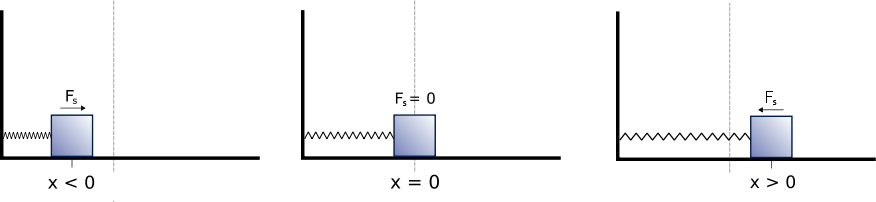
\includegraphics[scale=.5]{308px-Harmonic_oscillator.svg.png}
\caption{\simsun 一维谐振子}
\label{308px-Harmonic_oscillator.svg.png}
\end{figure}

令$\omega^2=\frac{k}{m}$(注意$\omega^2$的量纲:$[w^2]=\frac{\frac{kg\cdot m/s^2}{m}}{kg}=\frac{1}{s^2}$)得一维谐振子方程:
\[\frac{d^2x}{dt}+\omega^2x=0 \tag{*}\]

上式为二阶常系数齐次线性微分方程,这类方程的一般形式是
\[\frac{d^2x}{dt^2}+b\frac{dx}{dt}+cx=0\]
对于这类方程一般的解法如下:设$x(t)=e^{at}$,带入原方程得
\[(a^2+ba+c)e^{at}=0\]
上式称为原方程的特征方程,解得$a_1,a_2$,若$a_1\ne a_2$,则$e^{a_1t}$和$e^{a_2t}$就是原微分方程的两个彼此独立的解,方程的通解为它们的线性组合:
\[x(t)=c_1e^{a_1t}+c_2e^{a_2t}\]

考虑(*)式,它的特征方程是:
\[\lambda^2+\omega^2=0 \ \Rightarrow \  \lambda_1=\omega i\,, \lambda_2=\omega \]
\[ \therefore x_1(t)=e^{\omega i t},\,x_2(t)=e^{-\omega i t}\]
作$x_1(t),x_2(t)$的线性组合(由欧拉公式):
\[x_1'(t)=\frac{x_1+x_2}{2}=\cos\omega t\,,x_2'(t)=\frac{x_1-x_2}{2}=\sin\omega t\]
所以(*)的解为:
\[x(t)=c_1'x_1'+c_2'x_2'=A\cos(\omega t+\varphi)\]
其中$A$叫做\underline{振幅},$\varphi$叫做\underline{初相}。
\subsubsection{受阻下落}
设在空气中自由下落的物体受空气的阻力$\vec{F}$满足关系$\vec{F}=-\alpha\vec{v}$,则:
\[m\vec{a}=mg-\alpha\vec{v}\ \Rightarrow \ m\frac{d^2z}{dt^2}=mg-\alpha\frac{dz}{dt}\]
整理成标准形式
\[\frac{d^2z}{dt^2}+\frac{\alpha}{m}\frac{dz}{dt}=g\tag{**}\]
上式为二阶常数非齐次线性微分方程,它诱导的齐次微分方程如下:
\[\frac{d^2z}{dt^2}+\frac{\alpha}{m}\frac{dz}{dt}=0\]
设$z_1(t),z_2(t)$是上述齐次方程的两个独立的解,再设$z_s(t)$是方程(**)的一个特解,则方程(**)的一般解为
\[z(t)=z_s(t)+c_1z_1(t)+c_2z_2(t)\]
易解得$z_1=e^{-\frac{\alpha}{m}m},z_2=1$,再用以下方法求$z_s(t)$:设$z_s(t)=at$,代入(**)式:
\[\frac{\alpha}{m}a=g \ \Rightarrow\ a=\frac{mg}{\alpha}\]
\[\therefore z_s(t)=\frac{mg}{\alpha}t\]
综上所述:
\begin{align}
z&=c_1e^{-\frac{\alpha}{m}t}+c_2+\frac{mg}{\alpha}t \notag \\
&=c_1e^{-\frac{t}{\tau}}+c_2+v_ct\notag
\end{align}
由初始条件$t=0$时$z=0$得:
\[c_1+c_2=0\]
再由初始条件$t=0$时$\frac{dz}{dt}=0$,得:
\[-\frac{c_1}{\tau}+v_c=0\]
因此
\[c_1=v_0\tau,\,c_2=-v_c\tau\]
最终解得
\[z=v_c\tau\left(e^{-\frac{t}{\tau}}-1\right)+v_ct\]
\subsubsection{在太阳引力作用下讨论行星运动}
\begin{align}
\vec{F}&=-\frac{GMm}{r^2}\hat{r}=m\frac{d^2\vec{r}}{dt} \notag \\
\hat{r} &= \frac{x\vec{i}+y\vec{j}+z\vec{k}}{\sqrt{x^2+y^2+z^2}} \notag
\end{align}
可以证明,在有心力作用下质点做平面运动(见后)由于作用力为有心力,在平面极坐标系下考虑这个问题比较方便,此时外力只在$\vec{e_r}$方向有作用:
\[\begin{cases}
m(\ddot{r}-r\dot{\varphi}^2)=-\frac{GMm}{r^2}\\
m(2\dot{r}\dot{\varphi}+r\ddot{\varphi})=0
\end{cases}
\]
此为二阶非线性微分方程组,求解此方程组比较复杂,需利用方程组的两个初积分(或两个运动积分)
\[\begin{cases}
mr^2\dot{\varphi}=G_0,\,\text{角动量守恒}\\
\frac{1}{2}m(\dot{r}^2+r^2\dot{\varphi}^2)+V(r)=E,\text{机械能守恒}
\end{cases}
\]
得
\[
\frac{1}{2}m\dot{r}^2+V_{eff}(r)=E\,\text{其中第二项为有效势能}
\]
\[V_\text{eff}=\frac{G_0^2}{2mr^2}+V(r)\]
得
\[\dot{r}=\pm \sqrt{\frac{2}{m}[E-V_{eff}(r)]}\]
分离变数,得
\[dt=\frac{\pm dv}{\sqrt{\frac{2}{m}[E-V_{eff}(r)]}}\]
\[t=\int_{r_0}^r \frac{\pm dv}{\sqrt{\frac{2}{m}[E-V_{eff}(r)]}}\]
积分求得$r(t)$,再代入角动量守恒方程得
\[d\varphi = \frac{G_0 dt}{mr^2(t)}\]
求得
\[\varphi(t)=G_0\int_0^t \frac{dt}{mr^2(t)}+\varphi_0\]
在讨论太阳引力作用下行星的运动,其运动情况稍微简单一些。由运动方程组可推导出轨道微分方程,并求出其相应的轨道。
\subsection{初积分}
如果方程$G(x,y,z,\dot x,\dot y,\dot z,t)=c$对时间的一次微商是牛顿运动方程,就称上式为牛顿运动方程的初积分,或第一积分,从数学上看初积分使牛顿运动方程从二阶方程降为一阶方程,从物理上看,它表示某个力学量是运动守恒量。
\begin{align}
G_1&=r^2\dot\varphi=c \notag \\
\frac{G_2}{dt}&=2r\dot r\dot\varphi+r^2\ddot \varphi = r(2\dot r\dot\varphi+r\ddot\varphi)=0\notag \\
G_2&=\frac{1}{2}m(\dot r^2+r^2\dot{\varphi^2})-\frac{GMm}{r}=c_2 \notag \\
\frac{G_2}{dt}&=\frac{1}{2}m(2\dot r\ddot r+2 r \dot r \dot\varphi^2+2 r^2\dot\varphi\ddot\varphi)+\frac{GMm}{r^2}\dot{r}=0 \notag \\
\frac{G_2}{dt}&=\frac{1}{2}m(2\dot r\ddot r+2r \dot r \dot\varphi^2-4r\dot\varphi\dot r\dot\varphi)+\frac{GMm}{r^2}\dot{r}=0 \notag
\end{align}
\begin{align}
\dot r\left[ m(\ddot r-r\dot\varphi^2)+\frac{GMm}{r^2}\right]&=0 \notag \\
\frac{1}{2}m\dot r^2+\frac{mG^2}{2mr^2}-\frac{GMm}{r}&=c_2 \notag
\end{align}
\[ \Rightarrow r=\pm \sqrt{\frac{2}{m}\left[ c_2-\frac{c_1^2}{2r^2}+\frac{GMm}{r}\right] }\]
\section{质点在非惯性系中的运动、惯性力}
\subsection{非惯性系}
常常需要去非惯性参照系中讨论物体的运动,依照参照系变换时运动学量的变换关系,特别是加速度的变换关系,研究由惯性系中质量的运动方程推出非惯性参照系中质点的运动方程。

已知在惯性参照系中质点的运动服从牛顿第二定律
\[m\frac{d^2 \vec{r}}{dt^2}=\vec{F}\]
若已知非惯性参照系与惯性参照系的加速度的变换关系,例如:
\subsubsection{$S'$相对$S$作任意方式平动}由参照系变换公式和牛顿第二定律:
\[m(\vec{a'}+\vec{\omega})=\vec{F}\  \Rightarrow \ m\vec{a'}=\vec{F}-m\vec{\omega}=\vec{F}+\vec{F_i}\]

其中$\vec{F_i}$称作平移惯性力。
\subsubsection{$S'$相对$S$作匀角速度转动}由参照系变换公式和牛顿第二定律:
\[m(\vec{a'}+\vec{a_c}+\vec{a_{col}})=\vec{F}\]
\begin{align}
 \Rightarrow m\vec{a'}&=\vec{F}-m\vec{\omega}\times(\omega\times\vec{r'})-m2\vec{\omega}\times\vec{v'}\notag \\
 &=\vec{F}+\vec{F_c}+\vec{F_{col}}\notag \\
 &=\vec{F_{eff}} \notag
 \end{align}

其中 $\vec{F_c}$称作惯性离心力,$\vec{F_{col}}$称作科里奥利力,$\vec{F_{eff}}$称作表观力。可见在非惯性系下:\[ m\vec{a}=\vec{F_{eff}}\]

也即是在非惯性系中,质点的运动仍满足牛顿第二定律,只不过必须认为作用在质点的力除了真实的作用力$\vec{F}$外,还有虚拟的惯性力$\vec{F_i}$作用,即表观力的作用下的运动。

应该指出惯性力与真实力不同,无法指出惯性力的施力对象,也无法指出其反作用力,因此对惯性力无法涉及牛顿第三定律。但是在非惯性系中,在讨论质点运动时,它与真实力有着相同的效果。
\subsection{应用惯性力分析物理现象}
\subsubsection{在人造卫星或宇宙飞船绕地球运动时在舱内所看到的失重现象}
在人造地球卫星或宇宙飞船绕地球飞行时,卫星或飞船相对于地球有一心向加速度,在近地附近近似等于重力加速度。卫星或飞船参照系相对于地球的加速度也是这个加速度。因此在卫星参照系中物体所受的表观力(表观重力)为零,失重就是指的表观重力等于零(消失了)。
\begin{description}

\item[在地面上看]卫星以加速度$\vec{g}$绕地球转动:
\[m\vec{a}=m\vec{g}\]
\item[在卫星里看]在卫星里看,表观力为$0$,因此称为失重(但不是不受力):
\[m\vec{a'}=m\vec{g}+\vec{F_i}=m\vec{g}-m\vec{\omega}=0\]
\end{description}
\subsubsection{重力与纬度的关系}
\[\vec{F_i}=-m\vec{\omega}\times(\vec{\omega}\times\vec{r})\]
\[\vec{F_{eff}}=\vec{G}+\vec{F_i}=\vec{w}\]
\[\vec{F_i}:\text{惯性离心力}\]
\[\vec{G}:\text{地球引力(重力)}\]
\[\vec{w}:\text{表观重力}\]
$G=mg_0,F_i=m\omega^2 R cos\lambda,\omega$(地球自旋角速度)$=\frac{2\pi}{86400}\approx 7.29\times 10^{-5}/s,R$(地球半径)$\approx 6.4\times 10^6 m,\lambda:$纬度角
\begin{align}
w&=\sqrt{G^2+F_i^2-2GF_i \cos \lambda} \notag\\
&=G(1-\frac{F_i}{G}\cos\lambda\notag \\
&=mg_0(1-\frac{1}{289}\cos^2\lambda)\notag
\end{align}
\[\frac{\omega^2 R^3}{GM}=\frac{1}{289}\]
\[K=6.37\times 10^6m\, M=5.98\times 10^24kg\]
\[G=6.6726\times 10^{-11}m^3/kg\cdot s^2\]
令$w=mg$,
\[g=g_0(1-\frac{1}{289}\cos^2\lambda)\]
上式反映了重力$w$(因而重力加速度$g$)随纬度的变化。
\subsubsection{在地球上观测的科里奥利力}
科里奥利力:$\vec{F_{col}}=-2m\vec{\omega}\times\vec{v}=2m\vec{v}\times\vec{\omega}$

在北半球:河流对右岸冲击加剧;自由落体偏东;傅科摆。

有三个特征:
\begin{enumerate}
\item 与相对速度成正比,故只有当物体相对参照系运动时才可能出现;
\item 与转动参照系的加速度的一次方成正比,故当角速度较小时,科里奥利力比惯性离心力更重要
\item 力的方向总是与相对速度垂直,故不会改变相对速度大小,但却一定时时刻刻去改变运动的方向
\end{enumerate}

科里奥利力在地球上的表观:北半球:河流对右岸冲击加剧;火车对右轨的偏压较大;落体偏东;傅科摆。
\chapter{质点动力学(二)}
有了力的定律和牛顿定律,运动学的根本任务,即在一定环境下求解物体的运动问题,似乎就成为求解运动方程$m\ddot{\vec{r}}=\vec{F}(\vec{r},\dot{\vec{r}},t)$的数学问题了。但如果我们在动力学定律的基础上引进一些新的概念,如动量、角动量、动能、势能、机械能等,就可以进而得到关于这些量的新的规律。而直接用这些规律去分析质点的运动问题,往往比从牛顿定律出发更为方便。这些新的规律就是所谓运动定律以及由此列出的守恒定律。有时即使力的具体形式不十分清楚(如约束力,碰撞中质点间的作用力等)这种方法也能为我们求解问题提供一定信息。再者牛顿定律只适用质点,不能直接用于质点组,特别是由大量质点组成的体系,若我们用牛顿定律去求解体系中每个质点的运动,计算将十分复杂,甚至无法进行,而利用关于动量、角动量、能量的规律,却可以使我们不必求解每个质点运动的情况下,获得关于质点组运动的许多知识。事实上运动定理及守恒定律几乎是我们解决质点组动力学问题的唯一可以利用的工具。

关于动量、角动量、能量的运动定理以及守恒定律虽然最初是经典力学中由牛顿定律演绎出来的,但物理学的发展表明,动量、角动量、能量这些概念,有关它们的定理以及守恒定律却可以推广到物理学的其他领域,如研究电磁现象、热现象、量子现象,因而这些定理以及守恒定律有着更普遍的意义。

动量、角动量、能量等等这些力学量都可以视作状态量,或状态函数。以后在分析力学中引入的拉格朗日函数、哈密顿函数都可作为状态函数,不过是特别的状态函数(特性函数)。

质点由一种状态按照运动规律变为另一种\underline{状态},在物理学中称为一个过程。系统运动状态变化是由于一个过程中,系统与外界的相互作用(以及系统内部的相互作用)导致的,因此描述质点运动状态的物理量的改变是由过程中外界的作用(以及系统内部相互作用)过程所决定的。因此描述质点运动状态的物理量的改变,应该是有过程中外界的作用(以及系统内部相互作用)过程所决定的。即应该有状态量的改变=过程量。这就是著名的牛顿-莱布尼茨公示。
\begin{align}
\text{牛顿-莱布尼茨公式:}u(t_2)-u(t_2)&=\int_{t_1}^{t_2}f(t)dt\notag\\
\text{状态量的改变}&=\text{过程量}\notag
\end{align}
经典力学中有许多规律都可以表达为这种形式,许多重要的物理量也是通过类似的表达式引入的。下面我们将从牛顿的运动方程$m\frac{d^2\vec{r}}{dt^2}=\vec{F}$出发,讨论可以演绎出哪些类似的关系,并相应的引入新的物理量。

\section{动量、动量定理、动量守恒定律}
\subsection{动量、动量定理}
若质点的质量$m$为常数,则:
\[m\frac{d\vec{v}}{dt}=\vec{F}\ \Rightarrow\ \frac{d(m\vec{v})}{dt}=\vec{F}\]
令$\vec{p}=m\vec{v}$,则下式即为动量定理:
\begin{align}
\frac{d\vec{p}}{dt}&=\vec{F}\notag\\
\vec{p_2}-\vec{p_1}&=\int_{t_1}^{t_2}\vec{F}(t)dt=\vec{I_{12}}\notag\\
\text{动量的改变}&=\text{外力的冲量}\notag
\end{align}

其中$I_{12}$记作在$[t_1,t_2]$时间内外力的冲量。

质点在做匀速运动时,其惯性质量不再是常数。$m=m(\vec{v})$,但此时动量定理仍然适用。这说明在这种条件下牛顿方程必须修改,这一点也证明动量概念,动量定理较牛顿运动方程有更普遍的意义。我们将在后面狭义相对论部分进一步讨论这个问题。
\subsection{动量守恒定律}
若$\vec{F}(t)=0$,则:
\[I_{12}=\int_{t_1}^{t_2}\vec{F}dt=0\ \Rightarrow\ \vec{p_2}-\vec{p_1}=0\]
\[\vec{p}(t)=\vec{p}(0)=\vec{p_0}\]

动量守恒的概念在讨论质点组,特别是由两个质点组成的系统的运动问题时特别有用。若质点组织存在内部相互作用,由于牛顿第三定律,两个质点的相互作用的作用力和反作用力大小相等方向相反,$F_{12}=-F_{21}$,质点组各质点所受的总的冲量等于零,因此质点组的总动量$\vec{P}$守恒:
\[\vec{P}=(\vec{P_1}+\vec{P_2}+\dots)=\vec{P_0}\]

\subsection{动量定理、动量守恒定律应用于质点组}
\subsubsection{内力和外力、主矢量}
\begin{description}
\item[内力]质点组内任意两个质点之间的作用力,例如第$j$个质点对第$i$个质点有作用力,记作$\vec{F}_{ij}^{in}$;注意到由牛顿第三定律,$\vec{F}_{ij}^{in}=-\vec{F}_{ji}^{in}$
\item[外力]质点组任一质点所受的外界作用力,例如第$i$个质点受外界作用力,记作$\vec{F}_i^{ex}$
\item[主矢量]记作$\vec{F}^{ex}$,定义为$\vec{F}^{ex}=\sum_i \vec{F}_i^{ex}$
\end{description}
\subsubsection{质点组的总动量、质点组动量定理、总动量守恒}
\begin{description}
\item[总动量]记作$\vec{p}$,定义为$\vec{p}=\sum_i \vec{p_i}$
\item[质点组的动量定理]
\begin{align}
\frac{d\vec{p}}{dt} &=\sum_i \frac{d\vec{p_i}}{dt} = \sum_i (\vec{F}_i^{ex} + \sum_{j\ne i}\vec{F}_{ij}^{in}) \notag \\
&=\sum_i \vec{F}_i^{ex}+\sum_{ \substack{i,j \\ i\ne j}}\vec{F}_{ij}^{in} = \vec{F}^{ex} \notag
\end{align}
\[\frac{d\vec{p}}{dt}=\vec{F}^{ex}\ \Rightarrow\ \vec{p_2}-\vec{p_1}=\int_{t_1}^{t_2}\vec{F}^{ex}dt\]
\end{description}
\subsubsection{总动量守恒定律}
\[\text{若}\vec{F}^\text{ex}=0,\ \text{则}\vec{p_2}-\vec{p_1}=0\text{,总动量守恒}\]
\subsection{质心、质心运动定理、质心参照系}
\subsubsection{质心}(质量中心)$(M,\vec{r_c})$

质心是这样一个质点,它集中了质点组的全部质量,它的动量等于质点组的总动量
\[M=\sum_i m_i\]
\[\vec{p}=\sum_i \vec{p_i}=\sum m_i \frac{d\vec{r_i}}{dt}=\frac{d}{dt}(\sum_i m_i\vec{r_i})=M\frac{d\vec{r_c}}{dt}=M\vec{v_c}\]
\[\vec{r_c}=\frac{\sum_i m_i\vec{r_i}}{M}\text{表示质心的位置},\  v_c=\frac{d\vec{r_c}}{dt}\text{表示质心的速度}\]
\subsubsection{质点参照系}(对某一个质点组而言)
把原点取在质点上,坐标轴的方向始终与某一惯性系坐标轴保持平行的平动参照系叫做质点参照系,有时也称质点坐标系,或简称质心系。判断质心系是否是惯性系,只需判断质点系中的速度相对惯性系中是否为匀速。记$\vec{r_i'}$为相对质心系的位置矢量。

对于不受外力作用的体系(孤立系)或受外力的矢量和(主矢)为零的体系,其质心系为惯性系;否则,则为非惯性系。在讨论质点组动力学问题时,质心系具有一系列特点。在质心系中,质点组的总动量恒为零。
\begin{align}
\vec{r_i'}&=\vec{r_i}-\vec{r_c} \notag \\
\vec{v_i'}&=\vec{v_i}-\vec{v_c} \notag \\
\vec{p'}&=\sum_i m_i \vec{v_i'}=\sum_i m_i(\vec{v_i}-\vec{v_c}) = \vec{p}-M\vec{v_c}=0 \tag{*}
\end{align}
由(*)式可见,从质心系看,质点组的总动量恒为0
\subsubsection{质心系处理两体问题}
\subsection{例题分析}
\subsubsection{人船模型}
质量为$M=500kg$,长为$4m$的木船漂浮在静止的水面上,船尾站着一个质量为$50kg$的人,若人从船尾走到船头,问船相对于水面走了多少?
\begin{figure} [ht]
\centering

\includegraphics[scale=.6]{renchuan.png}
\caption{\simsun 人船模型}
\label{renchuan}
\end{figure}

\begin{enumerate}
\item 若船与水的摩擦力可以忽略,则此时人与船的总动量守恒
\[m\vec{v}+M\vec{v'}=0\]
\[\Rightarrow\int_{t_s}^{t_f}mvdt-\int_{t_s}^{t_f}Mv'dt=ml_1-Ml_2=0\]
因为是从船尾走到船头,所以人相对于船的位移为船长
\[L=l_1+l_2\]
因此
\[m(L-l_2)-Ml_2=0\]
\[\Rightarrow l_2=\frac{mL}{m+M}=\frac{4}{11}m\]
注意到船移动过程中,质心位移不变。
\item 若船与水的摩擦力不能忽略,并设阻力与船相对水的速度成正比,即$f=-\alpha\vec{v}$,并假设人以相对于船的恒定速率$v'$从船尾走到船头,分析船的运动可分为4个阶段:\begin{description}
\item[第一阶段]在极短的时间内,人从静止达到速度$v'$(相对船),同时船也从静止达到速度$V_{10}$,此阶段可忽略阻力(阻力的冲量趋近0),可用动量守恒。
\[m(v'+v_{10})+Mv_{10}=0\]
\item[第二阶段]人以速度$v'$(相对船)从船尾走到船头,此阶段必须考虑水的阻力的作用。
\[m\frac{d}{dt}(v'+v)+M\frac{dv}{dt}=-\alpha v\]
从$t=0$到$t=\frac{2}{v'}$求积分得到$v_{1f}$
\item[第三阶段]在极短的时间内,人在船尾定住,仿前,此阶段仍可忽略阻力,用动量守恒定律。
求$v_{20}$
\[m(v'+v_{1f})+Mv_{1f}=(m+M)v_{20}\]
\item[第四阶段]由于阻力的租用人和船一起由速度$V{20}$趋向速度$V_{2f}=0$
\[(m+M)\frac{dv}{dt}=-\alpha v\]
\end{description}
\end{enumerate}
\subsection{变质量物体的运动方程}
\subsubsection{体系的选择,主体,附体}
变质量物体运动过程分解为一系列元过程,在分析元过程时,在$\varDelta t$时间内由主体(设被考察变质量物体的质量为m),由于吸入(或抛开)附体(设其质量为$\varDelta m$)而合二为一(或一分为二)。
\subsubsection{变质量物体的运动过程}
\begin{align}
(m+\varDelta m)(\vec{v}+\vec{\varDelta v})-(\varDelta m\vec{u}+m\vec{v}) &= \vec{F}\varDelta t \notag \\
m\vec{v}+\varDelta m\vec{v}+m\vec{\varDelta v}+\varDelta m\vec{\varDelta v}-\varDelta m\vec{u}-m\vec{v}&= \vec{F}\varDelta t \notag \\
\end{align}
化简,舍去$\varDelta m\vec{\varDelta v}$这个二阶小量得
\begin{align}
m\vec{\varDelta v}+\varDelta m(\vec{v}-\vec{u})&=\vec{F}\varDelta t \notag \\
m\frac{d\vec{v}}{dt}+\frac{dm}{dt}(\vec{v}-\vec{u})&=\vec{F} \notag
\end{align}
\[\begin{cases}
\frac{dm}{dt}>0\quad\text{如:雨滴}\\
\frac{dm}{dt}<0\quad\text{如:火箭}\\
\end{cases}\]

\subsubsection{火箭的运动}
令$\vec{u}-\vec{v}=\vec{v_r}$,则$\vec{v_r}$表示燃料相对火箭的速度,若忽略$\vec{F}$的作用,运动方程为:
\begin{align}
m\frac{d\vec{v}}{dt}&=\vec{v_r}\frac{dm}{dt} \notag\\
mdv&=-v_rdm \notag\\
dv&=-v_r\frac{dm}{m} \notag\\
\int_{v_0}^{v_f}dv&=-v_r\int_{M_0}^{M_f}\frac{dm}{m} \notag\\
v_f-v_0&=-v_r(\ln M_f-\ln M_0)\notag\\
&=v_r\ln \frac{M_0}{M_f}=v_r \ln N\notag
\end{align}
最终结论为:
\[v_f-v_0=v_r\ln N\]
其中$N$为初末时刻的质量比,$N=\frac{M_0}{M_f}$;特别地,当$v_0=0$:
\[v_f=v_r\ln N\]
\[v_r \thickapprox
\begin{cases}
2km/s\text{,常规燃料}\\
4km/s\text{,非常规燃料}\\
\end{cases}\]
例如阿波罗三级火箭:
\begin{description}
\item[第一级] $v_{r_1}\thickapprox 2.9km/s,N_1=16$
\item[第二三级] $v_{r_2} \thickapprox 4km/s,N_2=14,N_3=12$
\[v_f=v{r_1}\ln N_1+v_{r_2}(\ln N_2+\ln N_3) = 28.5km/s\]

较著名的运载火箭
\begin{enumerate}
\item 中国:长征三号、长征四号
\item 美国:土星五号、大力神号
\item 欧洲:亚娜5型
\end{enumerate}

目前欧美的火箭已经能将有效载荷6吨以上送入地球同步轨道。
\end{description}
\section{动能与势能}
研究动力学问题,就要研究相互作用,既要看到里可以改变质点的动量(力的时间积累效应——冲量),也要看到里可以改变质点的动能(力的空间积累效应——功)。

对于质点组的动力学问题,既要研究质点组与外界的相互作用,也要研究质点组内部的相互作用。

质点组内部的相互作用,在许多情况下,如万有引力、弹性力、库仑力等都可以表示为两质点见相对位置的函数,这时体系内部相互作用力所做的功可以表述为体系的势能的改变。

这样对于质点组,除了上一节所介绍的动量概念外,还可以用动能,相互作用势能,机械能等等概念基于系统更细微,更完善的描述。而这些物理量的变化规律用动能定理,动能关系等等来表述。

质点组与外界相互作用时,既包含了动量的转移与交换(上一节内容),也包含了解量的转移与交换(本节内容),还包括了角动量的转移与交换(下一节内容),这样从不同层面反映了系统与外界相互作用时所包含的物理内容。

\[\text{动力学问题要研究的相互作用}
\begin{cases}
\text{力的时间积累效应(冲量)引起了动量的变化}\\
\text{力的空间积累效应引起了体系能量的变化}
\end{cases}\]
\subsection{动能、动能定理}
\subsubsection{质点的动能、动能定理}
\begin{align}
m\frac{d\vec{v}}{dt}=\vec{F} \ &\Rightarrow \ m\frac{d\vec{v}}{dt}\cdot\vec{v}=\vec{F}\cdot\vec{v} \notag\\
&\Rightarrow m(\frac{dv_x}{dt},\frac{dv_y}{dt},\frac{dv_z}{dt})\cdot(v_x,v_y,v_z)=\vec{F}\cdot\vec{v} \notag\\
&\Rightarrow \frac{d}{dt}(\frac{1}{2}m(v_x^2+v_y^2+v_z^2))=\vec{F}\cdot\vec{v} \notag\\
&\Rightarrow \frac{d}{dt}(\frac{1}{2}mv^2)=\vec{F}\cdot\vec{v} \notag\\
&\Rightarrow \frac{d}{dt}(E_k)=P \notag
\end{align}
\begin{align}
\varDelta E_k&=\underset{(c)}{\int_{\vec{r_1}}^{\vec{r_2}}}\vec{F}d\vec{r} \notag \\
\text{状态量的改变}&=\text{过程量}\notag
\end{align}
\subsubsection{功的计算}
定义元功:$dA=\vec{F}\cdot d\vec{r}$
\begin{align}
d\vec{r}&=dx\vec{i}+dy\vec{i}+dz\vec{k}\quad\text{(直角坐标系下)}\notag\\
dA&=F_xdx+F_ydy+f_zdz\notag\\
d\vec{r}&=dr\vec{e_r}+rd\theta\vec{e_\theta}+r\sin\theta d\varphi\vec{e\varphi}\quad\text{(球坐标系下)}\notag \\
dA&=F_rdr+F_\theta d\theta+F_\varphi r\sin\theta d\theta \notag
\end{align}
\begin{description}
\item[重力的功]
\[F_x=0 \quad F_y=0 \quad F_z=-mg \]
\begin{align}
F&=-mg\vec{k} \notag \\
dA&=-mgdz\notag\\
\int_a^b dA&=-mg\int_{z_a}^{z_b} dz\notag\\
&=-mg(z_b-z_a)\notag\\
&=mg(z_a-z_b)\notag
\end{align}
\item[万有引力的功]
\begin{align}
\vec{F}&=-\frac{GMm}{r^2}\vec{e_r}\notag\\
dA&=-\frac{GMm}{r^2}dr\notag\\
\int_a^b dA&=-\int_{r_a}^{r_b} \frac{GMm}{r^2} dr\notag\\
&= -GMm(-\frac{1}{r})|_{r_a}^{r_b}\notag\\
&=\frac{GMm}{r_b}-\frac{GMm}{r_a}\notag
\end{align}
\item[弹力的功的计算(一维情形)]
\begin{align}
\vec{F}&=-k\vec{x}=-kx\vec{i}\notag\\
dA&=-kxdx\notag\\
\int_a^b dA&=\int_{x_0}^{x_f}(-kx)dx\notag\\
&=-k(\frac{1}{2}x^2)|_{x_0}^{x_f}\notag\\
&=\frac{1}{2}kx_0^2-\frac{1}{2}kx_f^2\notag
\end{align}
\end{description}
\subsubsection{质点组动能、质点组动能定理}
\begin{description}
\item[质点组动能]\[E_k=\sum_i \frac{1}{2}m_iv_i^2\]
\item[质点组的动能定理]\[\frac{dE_k}{dt}=\sum_i \vec{F_i}\vec{v_i}\]
\begin{align}
E_{k_f}-E_{k_0}&=\sum_i A_i\notag\\
&= \sum_i \underset{(c)}{\int_{\vec{r_0}}^{\vec{r_f}}} \vec{F_i}d\vec{r_i} + \sum_{\substack{i,j\\i\ne j}}\vec{F}_{ij}^{in}\notag \\
&=A^{ex}+A^{in} \notag
\end{align}
\[A^{ex}=\sum_i \underset{(c)}{\int_{\vec{r_{i0}}}^{\vec{r_{if}}}}\vec{F}_i^{ex}d\vec{r_i}\]
\[A^{in}=\sum_i A_i^{in} = \sum_i\underset{(c)}{\int_{\vec{r_{i0}}}^{\vec{r_{if}}}}\sum_{\substack{i,j\\i\ne j}} \vec{F}_{ij}^{in} d\vec{r_i}\]
考虑第$i,j$个质点相互作用力所做的功:
\begin{align}
\vec{F}_{ij}^{in}d\vec{r_i}+\vec{F}_{ji}^{in}d\vec{r_j} &= \vec{F}_{ij}^{in}(d\vec{r_i}-d\vec{r_j}) \notag\\
&=\vec{F}_{ij}d\vec{r_{ji}}\notag
\end{align}\begin{align}
d\vec{r_i}+(\vec{r_{ij}}+d\vec{r_{ij}})+(-d\vec{r_j})+(-\vec{r_ij})&=0 \notag\\
d\vec{r_i}-d\vec{r_j}&=-d\vec{r_{ij}}\notag
\end{align}
\[\therefore A^{in}=\sum_{i<j}\underset{(c)}{\int_{\vec{r_{i0}}}^{\vec{r_{if}}}}\vec{F_{ij}}d\vec{r_{ji}} \]
\end{description}

作用力与反作用力这一对内力的总功只与两质点相对距离的变化$dr_{ij}$有关,在牛顿时空中,两质点相对距离的变化与参照系无关。因此内力的总共与参照系无关。

前面的例子,与其中一个质点相对静止的参照系中,作用于另一个质点的力仅与该质点的始末位置有关,而对该质点所经的具体路径无关。当然如果内力为耗散力就与路径有关了。
\subsection{质点组的势能}
\subsubsection{保守力和非保守力}
定义:作用在质点上的力$\vec{F}$,当质点由空间任一位置经过闭合路径$c$回到出发位置,$\vec{F}$所做的功恒为$0$,亦即
\[\oint\vec{F} d\vec{r}=0\]
则称$\vec{F}$为保守力,否则称非保守力。
\[\begin{cases}
\text{保守力如:万有引力,弹性力,库伦静电力}\\
\text{非保守力如:摩擦力($\oint \vec{F_\mu}d\vec{r}<0$),电路内的非静电力($\oint \vec{F}_\text{非静电力}d\vec{r}>0$)}
\end{cases}\]

保守体系:
若质点组内任一两质点间的作用力都是保守力,则称该质点组为保守体系。
\subsubsection{质点组的势能(两质点保守体系)}
设初始时两只点位置分别为$\vec{r_{10}},\vec{r_{20}}$,记为$\mathbf{a}=(\vec{r_{10}},\vec{r_{20}})$,经过一段时间,两质点分别到达位置$\vec{r_{1f}},\vec{r_{2f}}$,记为$\mathbf{b}=(\vec{r_{1f}},\vec{r_{2f}})$。由于两质点间的相互作用力,对两质点作的总功与路径无关,只与始末点位置有关,记为:\[A_{a\to b}\text{(保守力)} = -(E_p(\mathbf {a})-E_p(\mathbf {b}))\]
我们把$E_p(a),E_p(b)$称为质点组于位置$\mathbf{a}$和位置$\mathbf{b}$处的势能。由上式可知,$E_p(\mathbf{a}),E_p(\mathbf {b})$可差任一常数。保守力作用下两质点体系与这种与相对位置联系的做功本领称作保守体系的势能(或位能)。
\subsubsection{势能图,势能曲线}
\begin{description}
\item[势能图]表示势能与两质点相对位置关系的图形叫势能图
\item[势能曲线]若势能仅与相对位置的一个坐标有关,势能与该坐标的关系图形表示即为势能曲线
\begin{description}
\item[重力势能曲线]$\ $
\begin{figure} [ht]
\centering
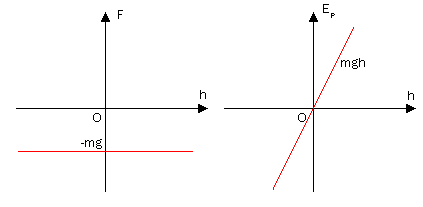
\includegraphics[scale=.6]{PotentialEnergy_Gravitational2.png}
\caption{\simsun 重力势能曲线}
\label{PotentialEnergy_Gravitational2}
\end{figure}
\item[弹力势能曲线]$\ $
\begin{figure} [ht]
\centering
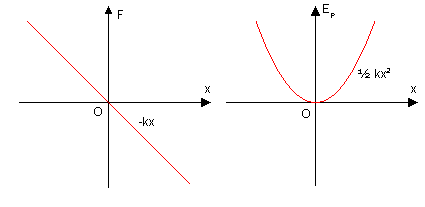
\includegraphics[scale=.6]{PotentialEnergy_Elastic.png}
\caption{\simsun 弹力势能曲线}
\label{PotentialEnergy_Elastic}
\end{figure}
\item[引力势能曲线] $\ $
\begin{figure} [ht]
\centering
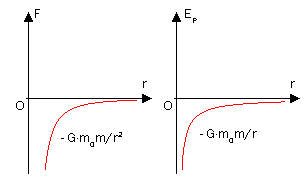
\includegraphics[scale=.6]{PotentialEnergy_Gravitational1.png}
\caption{\simsun 引力势能曲线}
\label{PotentialEnergy_Gravitational1}
\end{figure}
\item[双原子分子势能曲线]
\newpage
\begin{figure} [ht]
\centering
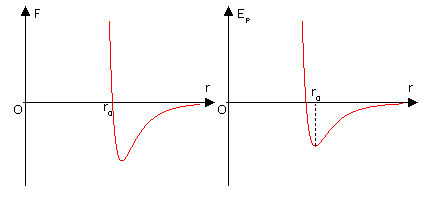
\includegraphics[scale=.6]{PotentialEnergy_Intermolecular.png}
\caption{\simsun 双原子分子势能曲线}
\label{PotentialEnergy_Intermolecular}
\end{figure}
\end{description}
\end{description}
\subsection{功能关系,机械能及其守恒定律}
\subsubsection{质点组的机械能,功能关系}
$A^{ex}$表示外力做功,则质点组的动能定理表述为:
\[E_{k_f}-E{k_0}=A^{ex}+A^{in}\]
\[A^\text{in}=A^\text{in}_\text{保守}+A^\text{in}_\text{非保守}\]
\[A^\text{in}_\text{保守} = -(E_{p_f}-E_{p_0})\]
\begin{align}
\therefore E_{k_f}-E_{k_0}&=-(E_{p_f}-E_{p_0})+A^\text{in}_\text{保守}+A^{ex} \notag \\
(E_{k_f}+E_{k_p})-(E_{k_0}+E_{p_0}) &= A^\text{in}_\text{保守}+A^{ex} \notag \\
E_f-E_0&= A^\text{in}_\text{保守}+A^{ex} \notag \\
\text{质点组的机械能之差}&=\text{外力的功}+\text{非保守内力的功}\notag
\end{align}
\subsubsection{机械能守恒}
若外力不做功($A^{ex}=0$)且非保守内力不做功($A^{in}_\text{非保守}=0$,没有动能转化为内能)则有
\[E_f-E_0=0\]
即
\[E_f=E_0=\text{恒量}\]
\subsubsection{$M\gg m$的两质点的孤立保守系的机械能守恒}
特点:
\begin{enumerate}
\item 机械能守恒:\[\frac{1}{2}MV^2+\frac{1}{2}mv^2+E_p(\vec{r}-\vec{R})=\text{恒量}\]
\item 质心系是惯性系:在质心系下
\[\begin{cases}
\vec{V}\ll\vec{v}:\quad M\vec{V}=-m\vec{v} \\
\vec{R}\ll \vec{r}:\quad M\vec{R}=-m\vec{r}
\end{cases}\]
\end{enumerate}
若$\frac{\frac{1}{2}MV^2}{\frac{1}{2}mv^2}=\frac{m}{M}(m\ll M)$,可以认为质心位置与$M$的位置相同,质点组的动能$=$小质点的动能。

设$E_p(\vec{r}_\text{相对})$表示在$M$产生的保守力场中的势能,此时:
\[\frac{1}{2}mv^2+E_p(\vec{r}_\text{相对})=\text{恒量}\]

即在质心系中,体系的动能表现为小质点的动能。体系的势能表现为仅由小质量质点的位置决定,即质量悬殊的两质点体系的机械能守恒表现为小指两质点的动能和势能之和为恒量。作为体系的另一部分,大质量质点在守恒定律表达式中似乎不出现。正是在这种意义下,我们会说到质点在保守力场中的机械能如机械能守恒定律。

在大质点物体($M$)的周围的空间,存在一种性质(物质),他表现为对外在着空间的任意位置的其他质点(其质量$m\ll M$)有力的作用,作用力的大小和方向完全有质量所在位置及其质量所决定,而且此力对质点所做的功仅有质点的始末位置决定,而与质点运动的具体路径无关。我们称这中间存在一种特殊的立场——保守立场,$M$是这力场的场源,而$M$对$m$的作用力则可称为保守立场对$m$的作用力。

地球对其表面附近物体的重力作用(重力场),地球对人造卫星的引力作用(引力场)都是保守力场,在原子物理中,氢原子中原子和对外围中子的静电力作用($M_p\gg m_e$)也属于保守立场。

对这样的体系的运动分析可归纳为单个质点在保守力场中的运动。

以及涉及质量在保守立场中的机械能以及机械能守恒定律

\[E=\frac{1}{2}mv^2+E_p=\text{恒量}\]

\subsubsection{质点在保守力场中机械能及其守恒定律}
\[\frac{1}{2}MV^2+\frac{1}{2}mv^2=\frac{1}{2}\mu(\vec{v}-\vec{V})^2\]
其中$\mu=\frac{Mm}{M+m}$称为约化质量。因为$\vec{v}\gg \vec{V}$,
\[\frac{1}{2}\mu (\vec{v}-\vec{V})^2+E_p(\vec{r}_\text{相对})=\frac{1}{2}\mu v^2+E_p(\vec{r}_\text{相对})=\text{恒量}\]

\subsection{质心系中的动能关系和机械能守恒定律}
\subsubsection{质心动能,柯尼希定理({\A Konig's theorem})}
设质点组各质点在某一参照系$S$的坐标为$\{\vec{r_i}\}$,在质心系$(c)$中的坐标用$\{\vec{r_i}'\}$表示,
\[\vec{r_i}=\vec{r_c}+\vec{r_i}' \quad \vec{v_i}=\vec{v_c}+\vec{v_i}'\]
\[E_k=\sum_i \frac{1}{2}m_i v_i^2 \quad E_{ck}=\frac{1}{2}MV_c^2\text{(质心在$S$系中的动能,$M=\sum_i m_i,\vec{r_c}=\frac{\sum_i m_i \vec{r_i}}{M}$)}\]
\[E_k=\sum_i \frac{1}{2}m_i v_i'^2\text{(质点组在质心系的动能)}\]
\[\text{三者关系:}E_k=E_{ck}+E_{kc}\]
\begin{theorem}[\simhei 柯尼希定理]
\simsun 质点系的总动能等于全部质量集中在质心时质心的动能,加上各质点相对于质心平动坐标系运动所具有的动能。
\end{theorem}
\begin{proof}[\simhei 证明]
\begin{align}
E_k=\sum_i \frac{1}{2}m_iv_i^2 &= \sum_i \frac{1}{2}m_i(\vec{v_c}+\vec{v_i}')(\vec{v_c}+\vec{v_i})\notag\\
&=\sum_i \frac{1}{2}m_i v_c^2+\sum_i \frac{1}{2}m_iv_i'^2+\sum_i \frac{1}{2}m_i 2\vec{v_c}\cdot\vec{v_i}'\notag
\end{align}
\begin{align}
\because&\ \sum_i \frac{1}{2}m_i2\vec{v_c}\cdot\vec{v_i}'=\vec{v_c}\cdot(\sum_i m_i\vec{v_i}')\text{\simsun ,在质心系中动量和为$0$}\notag\\
\therefore&\ \sum_i m_i\vec{v_i}'=0\notag\\
\therefore&\ \sum_i \frac{1}{2}m_i2\vec{v_c}\cdot\vec{v_i}'=0 \notag\\
\therefore&\ E_k=E_{ck}+E{kc}\notag
\end{align}
\end{proof}
\subsubsection{质心系中的动能关系和机械能守恒定律}
惯性参考系中:
\[E_f-E_0=A^{ex}+A^{in}_{\text{非保守}}\]
若质心系是惯性系:
\[E_f’-E_0‘=A^{ex}’+A^{in}_{\text{非保守}}‘\]
且若质心系是非惯性系时也成立,因为$A'_\text{惯性力}=0$,设质心对某惯性系的加速度$\vec{a}$,每一个质点在质心系中所受的惯性力为$-m_i\vec{a}$,惯性力所做的功
\[A'_\text{惯性力}=\sum_i(-m_i\vec{a})d\vec{r_i}=-\vec{a}\cdot(\sum_i m_i d\vec{r_i})=0\]
%\subsubsection{例题分析}
\subsection{碰撞}
\subsubsection{碰撞类型}
\[\begin{cases}\text{正碰,斜碰}\\
\text{弹性,非弹性碰撞}\begin{cases}\text{弹性碰撞:能量守恒}\\\text{非弹性碰撞:机械能损失}\begin{cases}
\text{一般非弹性碰撞}\\
\text{完全非弹性碰撞}
\end{cases}
\end{cases}
\end{cases}\]
\subsection{例题分析}

\section{角动量、角动量定理、角动量守恒定律}
这一节介绍另一个描述质点运动状态的物理量——角动量(又称动量矩)。当质点或体系作转动时,角动量是很重要的物理量。观察我们周围的世界,大到地球、太阳系、银河系、星系团,小到分子、原子,甚至是组成原子、分子的原子核、电子以及各层次的基本粒子,他们都在不停的“转动”着,而描述转动的最恰当的物理量是角动量。当体系有一个转动状态变为另一个转动状态,角动量要发生改变,这种改变由力矩、冲量矩决定,他们之间的联系由角动量定理来描述。

在物理世界中,常常遇到相互作用力是有心力的情况,有心力对力心的力矩、冲量矩等于零,因此在这种情况下,质点或系统关于力的角动量是守恒的,在宏观物理、微观物理中常常遇到这样的情况。
\begin{center}角动量是一个描述转动的物理量\end{center}
\subsection{角动量,角动量定理}
\[\frac{d\vec{p}}{dt}=\vec{F} \  \Rightarrow \ \vec{r}\times\frac{d\vec{p}}{dt}=\vec{r}\times\vec{F}\]
\[\text{注意到:}\frac{d}{dt}(\vec{r}\times\vec{p})=\frac{d\vec{r}}{dt}\times\vec{p}+\vec{r}\times\frac{d\vec{p}}{dt}=0+\vec{r}\times\frac{d\vec{p}}{dt}\]
\[\therefore \frac{d}{dt}(\vec{r}\times\vec{p}) = \vec{r}\times\vec{F}\]
定义$\vec{L}=\vec{r}\times\vec{p}$,称为质点相对于参考点$O$的角动量;定义$\vec{M}=\vec{r}\times\vec{F}$,称为质点所受外力相对于参考点$O$的力矩
\[\vec{L}=\vec{r}\times\vec{p}=m\vec{r}\times\frac{d\vec{r}}{dt}=2m\frac{d\sigma}{dt}\]
其中$\sigma$表示单位时间扫过的面积,$\vec{r}\times d\vec{r}=2d\sigma$,$\frac{d\sigma}{dt}$叫做面积速度;定义
\[\vec{L}=2m\vec{A}\]
$\vec{A}$称作面积速度
\[\vec{A}=\frac{d\sigma}{dt}\]
\subsection{质点组的角动量,质点组的角动量定理}
质点组的角动量定义为\[\vec{L}=\sum_i \vec{L_i}\]
\[\frac{d\vec{L}}{dt}=\sum_i \frac{dL_i}{dt}=\sum_i \vec{M_i} = \sum_i(\vec{M}_i^{ex}+\sum_{i\ne j} \vec{M}_{ij}^{in}) = \sum_i\vec{M}_i^{ex}\]
注意到$\sum_i \sum_{j\ne i} \vec{M_{ij}}^{in} = 0$
\[\vec{r_i}\times\vec{F_{ij}}+\vec{r_j}\times\vec{F_{ji}}=(\vec{r_i}-\vec{r_j})\times\vec{F_{ij}}=0\]
\[\Rightarrow \frac{d\vec{L}}{dt}=\sum_i \vec{M}_i^{ex}\]
\subsection{实验室系和质心系角动量之间的关系}
$\vec{L}=\vec{L_c}+\vec{L'}$
\[\vec{L}=\sum_i \vec{L_i},\vec{L_c}=\vec{r_c}\times\vec{p}=\vec{r_c}\times M\vec{v_0} = \sum_i \vec{r_i}\times\vec{p_i}\]
\[\vec{L'}=\sum_i \vec{L_i'}=\sum_i \vec{r_i'}\times\vec{p_i'}\]
\[\vec{r_i}=\vec{r_c}+\vec{r_i'},\vec{v_i}=\vec{v_c}+\vec{v_i'}\]
\begin{align}
\vec{L}&=\sum_i \vec{r_i}\times m\vec{v_i}=\sum_i (\vec{r_c}+\vec{r_i'})\times m(\vec{v_c}+\vec{v_i'})\notag \\
&=\vec{r_c}\times(\sum_i M_i\vec{r_i})+\sum_i \vec{r_c'}\times m \vec{v_i'}+\sum_i \vec{r_c}\times m_i \vec{v_i'}+\sum_i m_i \vec{r_i'}\times\vec{v_0} \notag \\
&=\vec{r_c}\times(\sum_i M_i\vec{r_i})+\sum_i \vec{r_c'}\times m \vec{v_i'}\notag
\end{align}
在质心系中$\sum_i m_i \vec{r_i'}=0,\sum_i m_i\vec{v_i'}=0$,推出
\[\vec{L}=\vec{L_c}+\vec{L'}\]
不论质心系是否是惯性系,在质心系中质点组的角动量定理仍然为
\[\frac{d\vec{L}'}{dt}=\sum_i \vec{M_i}^{ex}\quad(\sum_i \vec{M}_{i,\text{惯性}}=0)\]
\subsection{质点在有心力场中的运动}
\subsubsection{有心力、有心力场}
所谓有心力,就是方向始终指向(或被向)固定中心的力
\[\vec{F}=f(\vec{r})\vec{e_r}\]
$\vec{e_r}$为以固定中心为原点的矢径的单位矢量,而该固定中心成为力心。在大多数情况下,有心力的大小仅与考察点至力心的距离有关,即
\[\vec{F}=f(r)\vec{e_r}\]
这样的有心力称为中心对称有心力,这样的有心力是保守力,我们通常说的有心力指的就是这种中心对称的有心力。

前面去讨论$M\gg m$的二质点组成的保守体系时曾指出质心系与$M$静止参照系几乎等价。质心近似在$M$所在任意相互作用力,体系势能仅由$m$在$M$相对静止参照系中的位矢$\vec{r}$决定,可以推出:

在大质量周围的空间,存在一种性质(物质),他表现为对处于着空间的任意位置的其他质量(其质量$m\ll M$)有力的作用,作用力的大小和方向完全由质点所在位置及其性质(质量的,荷电量$q$等)所决定,我们称这空间存在一特殊的力场,$M$就是这力场的场源。若$M$对$m$的作用力是有心力,则称在$M$周围的空间存在有心力场。例如地球对其表面附近物体的重力作用,地球对人造卫星的引力作用,在原子中氢原子中原子核对外围电子的静电力作用,我们都可以表示为相应的对象在重力场、引力场、静电力场中所受的作用。而后两种情况都源于有心力场情形。
\subsubsection{有心力场中质点运动的一般特征——两个守恒量}
\begin{enumerate}
\item 角动量守恒:由于有心力对力心的力矩恒等于零
\[\vec{M}=\vec{r}\times f(r)\vec{e_r}=0\]
由质点角动量定理可知
\[\frac{d\vec{L}}{dt}=\vec{M}=0\quad \vec{L}=\vec{L_0}=\text{常量}\]
质点对于质心的角动量$\vec{L}$守恒
\[\vec{L}=\vec{r}\times\vec{p}=m\vec{r}\times\vec{v}=常矢量\]
$\vec{L}$的方向不变,质点必在由$\vec{r}\times\vec{v}$决定的平面内运动。

由此,讨论质点在有心力场中的运动,采用平面极坐标比较方便。$\vec{L}$的大小不变,$L=$常量。

在平面极坐标下,$\vec{v}=(\dot{r}\vec{e_r}+r\dot{\phi}\vec{e_{\phi}})$,$\vec{r}=r\vec{e_r}$
\[\vec{L}=\vec{r}\times\vec{p}=mr^2\dot{\phi} \vec{e_r}\times\vec{e_\phi}=mr^2\dot{\phi}\vec{k}\]
\[\vec{k}=\vec{e_r}\times\vec{e_\phi}\,\text{为垂直于质点轨道平面方向上单位矢量}\]
故有
\[L=mr^2\dot{\phi}=\text{常量}\]

\item 机械能守恒
由于有心力场是保守力场,可以引入势能函数$E_p$,由前,通常选择$r\to\infty$时为$E_p$的势能零点,则有
\[E_p^{(r)}=-\int_\infty^r f(r) dr = \int_r^\infty f(r) dr\]
例如在万有引力作用下$f(r)=-\frac{GMm}{r^2}$
\[E_p(r)=-\frac{GMm}{r}\]
在物理中常用$U$表示势能函数。

在有心力长中运动的质点机械能守恒,用平面极坐标系,$E_k=\frac{1}{2}m(\dot{r}^2+r^2\dot{\phi}^2)$

于是机械能守恒可表为
\[E_k+E_p=\frac{1}{2}m(\dot{r}^2+r^2\dot{\phi}^2)+U(r)=E=\text{常量}\]
在前面第二章中我们曾从运动方程出发讨论在太阳引力作用下行星的运动,由运动方程组
\[\begin{cases}
m(\ddot{r}-r\dot{\varphi}^2)=-\frac{GMm}{r^2}\\
m(2\dot{r}\dot{\varphi}+r\ddot{\varphi})=0
\end{cases}
\]
出发,先求出两个初积分
\[\begin{cases}
mr^2\dot{\phi}=G_0\\\
\frac{1}{2}m(\dot{r}^2+r^2\dot{\phi}^2)+V(r)=E
\end{cases}
\]
方程的两个初积分就是角动量守恒,机械能守恒。
\end{enumerate}
\subsubsection{有心力场中运动质点的轨道问题,轨道微分方程}
考虑到数学中一般习惯用$\nu$表示角度,以下讨论中我们用$\nu,\theta$取代$r,\phi$作为平面极坐标系中两个坐标变量,质点运动的轨道可以用函数$r(\theta)$来表示,为了求出$r(\theta)$满足的方程,我们可以从运动微分方程出发讨论
\[\begin{cases}
m(\ddot{r}-r\dot{\theta}^2)=F(r)\\
m(2\dot{r}\dot{\theta}+r\ddot{\theta})=0
\end{cases}
\]
也可以直接从方程的两个初积分,也就是两个守恒量出发讨论
\[\begin{cases}
mr^2\dot{\theta}=L\\\
\frac{1}{2}m(\dot{r}^2+r^2\dot{\theta}^2)+U(r)=E
\end{cases}
\]
下面我们从两个守恒量方程出发讨论,并以万有引力为例讨论

令$r^2\dot{\theta}=\frac{L}{m}=C$(两倍面积速度),并作变量替换$r\equiv\frac{1}{u}$,则有
\[\dot{\theta}=cu^2\]
\[\dot{r}=\frac{dr}{d\theta}\dot{\theta}==-C\frac{du}{d\theta}\]
在万有引力下
\[U=-\frac{GMm}{r}=-GMmu\]
代人机械能守恒方程得
\[\frac{1}{2}mc^2\left[(\frac{du}{d\theta})^2+u^2\right]-GMmu=E\]
整理后得
\[(\frac{du}{d\theta})^2=A^2-(B-u)^2\]
其中$B\equiv \frac{GM}{c^2},A^2=\frac{2E}{mc^2}+\frac{G^2M^2}{c^4}$

将上式开方,并分离变数得
\[\frac{du}{\sqrt{A^2-(B-u)^2}}=\pm d\theta\]
积分后得
\[\cos^{-1}(\frac{u-B}{A})=\pm \theta+\alpha\]
因此得轨道方程
\[u=B+A\cos(\theta-\beta)\]
上式已把积分常量$\mp \alpha$换成另一个常量$\beta$,回到$r(\theta)$的形式,得
\[r=\frac{\frac{1}{B}}{1+\frac{A}{B}\cos(\theta-\beta)}=\frac{P}{1+e\cos(\theta-\beta)}\]
这是圆锥曲线方程
\[p\equiv \frac{1}{B}=\frac{c^2}{GM}\,\text{半正焦距}\]
\[e=|\frac{A}{B}|=\sqrt{1+\frac{2Ec^2}{G^2M^2m}}\,\text{偏心率}\]
$P,e$由两个状态参量$E$和$C$(也是两个守恒量)决定,它们可由初条件$(\vec{r_0},\vec{v_0})$确定。
\[E<0\quad e<1\quad \text{椭圆}\]
\[E=0\quad e=1\quad \text{抛物线}\]
\[E>0\quad e>1\quad \text{双曲线}\]
\[C=\sqrt{GMP}\]
\[E=\frac{GMm}{2P}(e^2-1)=-\frac{GMm}{2a}\quad\text{(若$e<1$)}\]
$a$为轨道半长轴,$b=a\sqrt{1-e^2}$
\[(e=\frac{c}{a}\, P=\frac{b^2}{a}\, e=\sqrt{a^2-b^2}\, P=a(1-e^2)\, b=a\sqrt{1-e^2})\]
可见机械能$E$与半长轴$a$直接有关系,而角动量$L$(因而$C$)与半正焦距$P$直接有关。
\subsubsection{附:开普勒三大定律}
\begin{enumerate}
\item 第一定律(椭圆轨道),行星沿椭圆轨道绕太阳运行,太阳位于椭圆的一个焦点上。
\item 第二定律(面积定律),对于任一个行星而言,它的矢径在相同的时间内扫过相等的面积
\item 第三定律(周期定律 ),行星绕太阳运动轨道半长轴$a$的立方与周期$T$的平方成正比。$\frac{R^3}{T^2}=$常数$K$,$K=\frac{GM}{4\pi^2}$称为太阳系常量。注意$[K]=[GM]=L^3T^{-2}$
\end{enumerate}

开普勒第一定律、第二定律发表于1609年,第三定律则发表于1618年。有趣的是,开普勒定律的发现在前,而微积分技术、牛顿的力学定律如万有引力定律发现在后,微积分技术发现于十七世纪中叶,而牛顿的《自然哲学的数学原理》发表于1687年,是物理学史上第一次大综合。是天文学、数学、力学历史发展的产物,也是牛顿创造性研究的结晶。
%\subsection{例题分析}
\section{运动定理及守恒定律小结}
为了更深入研究物体的机械运动引进了一些新的物理量,包括描述物体运动状态的物理量如描述外界对物体作用的物理量,并得到了有关物理量的运动定理以及守恒定律。
\subsection{基本概念}
\begin{center}
动量、角动量、动能、势能(仅对质点组而言)、机械能、力、冲量、力矩、冲量矩、功、功率\\
(仅对质点组而言)外力、内力、保守内力、非保守内力\\
(对质心组)质心、质心动量、质心角动量、质心动能、质心系\\
\end{center}
\subsection{基本规律}
\subsubsection{质点动量定理}
 \[\frac{d\vec{p}}{dt}=\vec{F}\]
\[ \vec{p}-\vec{p_0}=\int_0^t\vec{F}dt=I\text{(冲量)} \]
质点组动量定理:\[\frac{\vec{p}}{dt}=\vec{F}^\text{ex}\]
动量守恒定律:若$\vec{F}^\text{ex}=0$(质点组),或者内部作用强烈、发生时间短促时\[\vec{p}=\vec{p_0}\]
\subsubsection{角动量定理}
质点角动量定理:\[\frac{d\vec{L}}{dt}=\vec{M}\]\[\vec{L}=\vec{r}\times\vec{p},\vec{M}=\vec{r}\times\vec{F}\]
质点组角动量定理:\[\frac{d\vec{L}}{dt}=\vec{M}^\text{ex}\]
角动量守恒定律:若$\vec{M}^\text{ex}=0$,则\[\vec{L}=\vec{L_0}\]
\subsubsection{动能定理}
质点动能定理:\[E_k-E_{k_0}=A\]
其中$A$为外力的功
\[A=\underset{(c)}{\int_a^b}\vec{F}d\vec{r}\]
质点组动能定理:
\[E_k-E_{k_0}=A^\text{ex}+A^\text{in}\]其中\[A^\text{in}=A^\text{in}_\text{保守}+A^\text{in}_\text{非保守}\]
\subsubsection{保守内力、体系势能}
保守内力:即$\oint\vec{F}d\vec{r}=0$(沿任何闭合路径力的积分为0),如重力、弹性力、万有引力

体系势能:\[E_p(b)-E_p(a)=-\int_a^b\vec{F}d\vec{r}\quad\text{(沿任意一条路径)}\]
\subsubsection{质点组机械能守恒定律}
\[E=E_k+E_p\]
功能关系:\[E-E_0=A^\text{ex}+A^\text{in}_\text{非保守}\]
若$A^\text{ex}=0$,$A^\text{in}_\text{非保守}=0$,则机械能守恒,$E=E_0$。

\chapter{振动和波}
\section{简谐振动}
\section{阻尼振动和受迫振动}
\section{振动的合成与分解}
\section{机械波的产生和传播}
\section{平面简谐波}
\section{弹性介质中的波动方程与波速}
\section{波的能量和强度}
\section{驻波}
\section{多普勒效应}

\chapter{相对论简介}
\section{相对论运动学}
\subsection{四维空间;事件;间隔;间隔不变性}
\textbf{四维时空:}时间和空间构成统一整体,成为四维时空。有时称为四维闵可夫斯基空间。\\
\textbf{事件:}四维时空中一点,某时某地。\\
\textbf{例如}\\
$$
\begin{array}{lll}
 &\text{在系中}&\text{在系中}\\
\text{事件}A&(t_{1},x_{1},y_{1},z_{1})&(t_{1}',x_{1}',y_{1}',z_{1}')\\
\text{事件}B&(t_{2},x_{2},y_{2},z_{2})&(t_{2}',x_{2}',y_{2}',z_{2}')
\end{array}
$$
两个事件~A.B 之间的间隔\\
$$
\begin{array}{lcc}
\text{时间间隔}&\Delta t&\Delta t'\\
\text{空间间隔}&\Delta l=\sqrt{\Delta x)^{2}+(\Delta y)^{2}+(\Delta z)^{2}}&\Delta l'=\sqrt{\Delta x')^{2}+(\Delta y')^{2}+(\Delta z')^{2}}
\end{array}
$$
间隔$$(\Delta s)^{2}=c^{2}\Delta t^{2}-[(\Delta x)^{2}+(\Delta y)^{2}+(\Delta z)^{2}]$$
间隔不变性:两个事件之间的间隔与不同惯性参照系中是相等的‘
$$(\Delta s)^{2}=(\Delta s')^{2}$$
即$$c^{2}\Delta t^{2}-[(\Delta x)^{2}+(\Delta y)^{2}+(\Delta z)^{2}]=c^{2}\Delta t'^{2}-[(\Delta x')^{2}+(\Delta y')^{2}+(\Delta z')^{2}]$$
间隔不变性是真空中光速不变原理的数字体现。
间隔的分类:
$$
\begin{array}{cc}
(\Delta s)^{2}>0&\text{类时间隔}\\
(\Delta s)^{2}=0&\text{类光间隔}\\
(\Delta s)^{2}<0&\text{类空间隔}
\end{array}
$$
\subsection{洛伦兹变换}
洛伦兹变换是洛伦兹在1892 年为了解决电磁学理论的协变形问题而提出的变换关系。\\
设惯性参照系$\sum'$ 相对惯性参照系$\sum$ 以速度v 沿$x(x)'$ 轴作匀速直线运动。\\
引入四维时空的坐标\ \ $x^{\alpha},\ \ \alpha=0,1,2,3$\\
$${x^{\alpha}}=(ct,x,y,z)$$
一个事件A 在$\sum$ 系和$\sum'$ 系中的坐标分别为\{ $x^{\alpha}$ \}和\{ $x'^{\alpha}$ \}\\
参照系变换时,时空坐标的变换用下列矩阵关系来描述\\
其中\\
\ \ \ $\beta \equiv \frac{v}{c},\ \ \ \gamma \equiv \frac{1}{\sqrt{1-\beta^{2}}}$
写成分量表达式即为\\

$$
\begin{array}{lcl}
ct'&=&r(ct-\beta x)\\
x'&=&r(x-\beta ct)\\
y'&=&y\\
z'&=&z
\end{array}
$$
上述~$\sum$ 系,$\sum'$ 系中坐标变换关系式称为洛伦兹变换。这个变换虽然是在爱因斯坦提出完整的狭义相对论理论之前提出的,但是它对狭义相对论的建立有这只管种烟的启发作用,而且成了狭义相对论理论的重要组成部分。\\
\\
洛伦兹包含了以下一些重要的内容:\\
\begin{enumerate}
\item 相比有伽利略变化所包含的绝对时间观念~$t'=t$,狭义相对论中不同的参照系中有不同的时间,与参照系之间的相对运动有关。
\item 在洛伦兹变换下,两个事件~A.B 之间的间隔保持不变。\\
$$
\begin{array}{rcl}
(\Delta s')^{2}&=&(\Delta s)^{2}\\
c^{2}\Delta t'^{2}-[(\Delta x')^{2}+(\Delta y')^{2}+(\Delta z')^{2}]&=&c^{2}\Delta t^{2}-[(\Delta x)^{2}+(\Delta y)^{2}+(\Delta z)^{2}]
\end{array}
$$
事实上
$$
\begin{array}{rcl}
c^{2}(\Delta t')^{2}&=&r^{2}(c\Delta t-\beta (\Delta x))^{2}\\
(\Delta x')^{2}&=&r^{2}(\Delta x-\beta c(\Delta t))^{2}\\
(\Delta y')^{2}&=&(\Delta y)^{2}\\
(\Delta z')^{2}&=&(\Delta z)^{2}\\
c^{2}(\Delta t')^{2}-(\Delta x')^{2}&=&r^{2}(c\Delta t-\beta (\Delta x))^{2}-r^{2}(\Delta x-\beta c(\Delta t))^{2}\\
&=&r^{2}(1-\beta^{2})c^{2}(\Delta t)^{2}-r^{2}(1-\beta^{2})(\Delta x)^{2}\\
&=&c^{2}(\Delta t)^{2}-(\Delta x)^{2}
\end{array}
$$
\item 在洛伦兹变换下,有下述速度变换关系是
$$
\begin{array}{rcccl}
u'_{x}&=&\frac{dx'}{dt'}&=\frac{u_{x}-v}{1-\frac{v}{c^{2}}u_{x}}\\
u'_{y}&=&\frac{dy'}{dt'}&=\frac{u_{y}}{1-\frac{v}{c^{2}}u_{x}}\sqrt{1-\frac{v^{2}}{c^{2}}}\\
u'_{z}&=&\frac{dz'}{dt'}&=\frac{u_{z}}{1-\frac{v}{c^{2}}u_{x}}\sqrt{1-\frac{v^{2}}{c^{2}}}\\
\end{array}
$$
即速度矢量(三维空间矢量)不在描述原来的速度公式法则。\\
可以证明光速在洛伦兹变换下保持不变,而小于~c 的速度在洛伦兹变换下永远不会达到或超过~c(这一点也可用间隔得不变性来论证)。\\
\item 在非相对论极限下($\beta\ll 1, \gamma\approx 1$)\\
洛伦兹变换退化为伽利略变换\\
\end{enumerate}

\subsection{洛伦兹变换下的标量、矢量、  }
\subsubsection{狭义相对性原理及其数学体现}
\textbf{狭义相对性原理:}一切物理规律在任何惯性系都应有相同的形式。\\
\textbf{一切物理规律:}电磁学规律、力学规律、强行互作用规律、弱相互作用规律。(引力相互作用具有特殊性,引力效应与时空结构密切相关——广义相对论)\\
\textbf{对于任何惯性系都应有相同形式:}惯性系之间的变换用洛伦兹变换描述,用以表示物理规律的方程在洛伦兹变换下应保持其形式不变,常把方程的这一性质称之为具有协变性。\\
\subsubsection{洛伦兹变换下的标量、矢量、张量  }
\begin{enumerate}
\item 普遍的洛伦兹变换:\\
凡是使四维时空中两个事件之间的间隔\\
$$(\Delta s)^{2}=c^{2}\Delta t^{2}-[(\Delta x)^{2}+(\Delta y)^{2}+(\Delta z)^{2}]$$
保持形式不变的线性变换统称为普遍的洛伦兹变换。
$$x'^{\alpha}=\sum_{\beta}\Lambda^{\alpha}_{\beta}x^{\beta}\equiv\Lambda^{\alpha}_{\beta}x^{\beta}$$
前面所描述的一个惯性系~$\Sigma'$ 相对另一惯性系~$\Sigma$ 沿~$x(x')$ 轴做匀速直线运动时,两个参照系时空坐标的变换只是普遍的洛伦兹变换的一种特殊性,常称之为特殊的洛伦兹变换。普通的洛伦兹变换还包括:空间转动、空间反演、时间反演、空间时间全反演等。洛伦兹变换具有群的结构。\\
\item 四维闵可夫斯基空间中的标量、矢量、张量。\\
狭义相对论下的四维时空是一个与欧式空间具有不同度量特征的空间。其度量张量常表示为\\



两个事件之间的间隔用上述度规张量(常称为闵可夫斯基度规)来表示可写为
$$ds^{2}=\sum_{\alpha.\beta}\eta_{\alpha}dx^{\alpha}dx^{\beta}$$
或者按照爱因斯坦约定在表达式中若两指表重复则意味着对该指标求和,可写为
$$ds^{2}=\eta_{\alpha\beta}dx^{\alpha}dx^{\beta}$$
所以狭义相对论的四维时空又称为四维闵可科夫斯基空间。\\
四维闵可夫斯基空间中的各种物理量。各种微分算子可以按其在洛伦兹变换下的变换性质将其分类。标量、矢量、张量、等。我们称这些在洛伦兹变换下的协变形式的量成为协变量。\\
\begin{enumerate}
\item 标量$\Phi$
一个量只有一个分量。在洛伦兹变换下保持不变,称为标量\\
例如:\\
两个事件之间的间隔$ds^{2}$
$$
\begin{array}{rcl}
ds^{2}&=&\eta_{\alpha\beta}dx^{\alpha}dx^{\beta}\\
&=&c^{2} dt^{2}-[(dx)^{2}+(dy)^{2}+(dz)^{2}]
\end{array}
$$
又如:运动粒子的固有时$\tau$ ,在相对粒子局域静止测定的时间间隔。\\
$$
\begin{array}{rcccl}
d\tau & \equiv & \frac{1}{c}ds & = & \frac{1}{c}(cdt\sqrt{1-\frac{u^{2}}{c^{2}}})\\
 & = &\frac{dt}{r_{u}} & &
\end{array}
$$
u为粒子的瞬时速度$r_{u}=\frac{1}{\sqrt{1-\frac{u^{2}}{c^{2}}}}$
\item 矢量$\{\bigvee^{\alpha}\}$\\
一个量由4个分量组成$\bigvee^{\alpha} \ \ (\alpha=0,1,2,3)$在洛伦兹变换下如同时空坐标变换一样变换。
$$V'^{\alpha}=\Lambda^{\alpha}_{\beta}V^{\beta}\ \ \ (\alpha=\beta=0,1,2,3)$$
如:四位移$dx^{\alpha}$\\
又如:四速度矢量$u^{\alpha}$
$$\{U^{\alpha}\}\equiv\{\frac{dx^{\alpha}}{d\tau}\}=r_{u}(c,u_{1},u_{2},u_{3})=r_{u}(c,\overrightarrow{u})$$
又如:四维动量$p^{\alpha}$
$$p^{\alpha}=m_{0}U^{\alpha}$$
$m_{0}$为粒子的静止质量,是四维闵可夫斯基空间中的标量。\\
上式也可写为$$\{p^{\alpha}\}=(p^{0}, \overrightarrow{p})$$
若引入$m\equiv r_{u}\equiv m_{0}$ 粒子的惯性质量
$$p^{0}=mc\ \ \ \ \ \ \ \ \ \overrightarrow{p}=m\overrightarrow{u}$$
$p^{0}$与粒子的能量E有如下关系$p^{0}=\frac{E}{C}$\\
故有 $E=p^{0}c=mc^{2}$
\item 二阶张量$T^{\alpha\beta}$\\
一个量$\{T^{\alpha\beta}\}$具有$4\times4=16$个分量,在洛伦兹变换下按如下方式变换。
$$T'^{\alpha\delta}=\Lambda^{\lambda}_{\alpha}\Lambda^{\delta}_{\beta}T^{\alpha\beta}$$
称为二阶张量。\\
以后在电磁学理论中可以看到电场强度$\overrightarrow{E}$和磁感应强度$\overrightarrow{B}$一起构成电磁场场张量$F^{\alpha\beta}$它是二阶(反对称张量)\\
\item 微分算子\\
标量微分算子$\frac{d}{d\tau}$\\
矢量微分算子$\{\frac{\partial}{\partial x^{\alpha}}\}=\{\frac{1}{c}\frac{\partial}{\partial t},\frac{\partial}{\partial x},\frac{\partial}{\partial y},\frac{\partial}{\partial z}\}$\\
波算子$\Box^{2}=-\frac{1}{c^{2}}\frac{\partial^{2}}{\partial t^{2}}+\frac{\partial^{2}}{\partial x^{2}}+\frac{\partial^{2}}{\partial y^{2}}+\frac{\partial^{2}}{\partial z^{2}}$\\
也是标量算子。
\end{enumerate}
\end{enumerate}
\section{相对论动力学}
牛顿力学是非相对论力学,其运动方程为三维形式,要将其改造为相对论力学,必须将其四维协变形式,从而满足相对性原理的要求。在经典力学中我们有牛顿运动方程$\frac{\overrightarrow{p}}{dt}=\overrightarrow{F}$,也有能量随时间变化的规律$\frac{dE}{dt}=\overrightarrow{F}\cdot\overrightarrow{v}$,在一定条件下,我们有动量守恒定律,也有能量守恒定律。我们将把这些规律进行综合改造。找出满足相对论要求的协变形式。
\subsection{四维动量$p^{\alpha}$(能量-动量四维矢量)\\四维动量守恒(能量-动量守恒)}
由前,在狭义相对论中引入四维动量
$$p^{\alpha}=m_{0}U^{\alpha}$$
$m_{0}$:静止质量。闵可夫斯基空间中的标量。
$$U^{\alpha}=(\gamma_{u}c,\gamma_{u}\overrightarrow{u})\ \ \ \ \ r_{u}=\frac{1}{\sqrt{1-\frac{u^{2}}{c^{2}}}}$$
其空间分量$\overrightarrow{p}=m_{0}\gamma_{u}\overrightarrow{u}=\frac{m_{0}\overrightarrow{u}}{\sqrt{1-\frac{u^{2}}{c^{2}}}}\equiv m\overrightarrow{u}$\\
$m\equiv\gamma_{u}m_{0}=\frac{m_{0}}{\sqrt{1-\frac{u^{2}}{c^{2}}}}$\ \ \ \ m:动质量,惯性质量。
$$m\rightarrow\infty(u\rightarrow c)$$
m随粒子运动状态变化而变化,当u增大时,粒子的惯性增大。$u\rightarrow c$时,惯性无穷大。\\
早在1901年考夫曼在实验中发现,高速粒子的荷质比$\frac{e}{m}$随速率的增大而减小。根据电荷守恒定律, 质量电子电荷不随电子运动速率变化,(源自的电中性量其佐证)于是他得出了质量m随速率增大而增大的结论。先带学的实验也证实动量$p=m\overrightarrow{v}$随着粒子的速度接近光速$(\frac{u}{c}\rightarrow1)$而迅速增大。\\
时间分量
$$
\begin{array}{rcl}
p^{0}&=&\gamma_{u}m_{0}c\\
&=&\frac{1}{c}\frac{m_{0}c^{2}}{\sqrt{1-\frac{u^{2}}{c^{2}}}}\\
&=&\frac{1}{c}(m_{0}c^{2}+\frac{1}{2}m_{0}u^{2}+\cdot\cdot\cdot)\\
&\equiv&\frac{E}{C}
\end{array}
$$
$E\equiv\gamma_{u}m_{0}c^{2}=mc^{2}$\ \ \ \ \ 质量关系式\\
质能关系式是现代核能反应中或释放能量,或吸收能量,其依据也是质能关系式。
$$E_{k}=\Delta E=(\Delta m)c^{2}$$
若粒子的静止质量为零($m_{0}=0$),如光子,某些中微子其四动量通常用$q^{\alpha}$表示\\
$$q^{\alpha}=(q,\overrightarrow{q})\ \ \ \ \ E=qc$$
可证:$$\eta_{\alpha\beta}q^{\alpha}q^{\beta}=0(=m_{0}c^{2})$$
四动量守恒(能量-动量守恒)\\
在粒子参与的各种碰撞的反应过程中,反应前后的四动量之和保持不变。
$$\sum_{i}P_{i}^{\alpha}=\sum_{j} P_{j}'^{\alpha}$$

例:带电$\pi$介子(不稳定介子)可 衰变  为$\mu$  子和中微子
$$\pi^{+}\rightarrow\mu^{+}+\gamma_{\mu}$$
上述衰变过程中所涉及的粒子的静止质量分别为
$$
m_{\pi}=139.57Mev/c^{2}$$$$m_{\mu}=105.66Mev/c^{2}$$$$m_{\nu}\approx0 $$(即使有亦很小)
$$(1Mev=1.6\times10^{-13}J,\ \ 1Mev/c^{2}=1.78\times10^{-30}Kg)$$
求衰变后的$\mu$子在$\pi$介子质心系中的能量、动量和速度。\\
解:\ \ \ 在$\pi$介子质心系中,$\pi$介子的动量、能量为
$$P=0,\ \ \ \ E=m_{\pi}e^{2}$$
设$\overrightarrow{P}'_{(\mu)}$和$\overrightarrow{P}'_{(\nu)}$分别是$\mu$介子和中微子的动量,它们的能量分别是
$$E'_{()\mu}=\sqrt{m^{2}_{\mu}c^{4}}=p'^{2}_{(\mu)}c^{2}\ \ \ E'_{(\nu)}=P'_{(\nu)}c$$
有四动量守恒得\\
动量守恒:$\overrightarrow{P'_{(\mu)}}+\overrightarrow{P'_{(\nu)}}=0$\\
能量守恒:$\sqrt{P_{(\mu)}'^{2}\cdot c^{4}+P_{(\mu)}c'^{2}}+P'_{(\nu)}c=m_{\pi}c^{2}$
由上面第一式得:$\mid \overrightarrow{P'_{(\mu)}}\mid=\mid \overrightarrow{P'_{(\nu)}}\mid=P'$
代入第二式解得:$P'=\frac{m_{\pi}^{2}-m_{\mu}^{2}}{2m_{\pi}}c$
$$E'_{(\mu)}=m_{\pi}c^{2}-P'c=\frac{m_{\pi}^{2}+m_{\mu}^{2}}{2m_{\pi}}c^{2}$$
把粒子质量带入得:$$P'=29.79Mev/c\ \ \ \ E'_{(\mu)}=109.78Mev$$
$\mu$子 $\gamma$ 子为$\gamma=\frac{1}{\sqrt{1-\frac{u^{2}}{c^{2}}}}=\frac{E'_{\mu}}{m_{\mu}c^{2}}=1.0390$
由此求得$\mu$子的速度为$\mu=0.2714c$
\subsection{相对论力学方程}
如前所述,要是力学规律满足相对性原理要求必须使其具有四维协变形式。前面所述的四维动量及四动量守恒定率即是四维协变形式。同样相对论动力学的运动方程也必须是四维协变形式。\\
牛顿运动方程$\frac{d\overrightarrow{P}}{dt}=\overrightarrow{F}$,是三维形式。不难猜测,相应的四维形式应该是$$\frac{dP^{\alpha}}{d\tau}=K^{\alpha}$$
其中$P^{\alpha}$为四维动量$d\tau$是固有市它的微分    $K^{\alpha}$通畅称谓四维力。$K^{\alpha}=\{K^{0},\overrightarrow{K}\}$\\
其空间分量:$\overrightarrow{K}=\frac{d\overrightarrow{p}}{d\tau}=\gamma\frac{d\overrightarrow{p}}{dt}=\gamma\overrightarrow{F}$
时间分量\ :$K^{0}=\frac{dp^{0}}{d\tau}=\gamma\frac{d}{dt}(\frac{E}{C})=\gamma\frac{\overrightarrow{F}\cdot\overrightarrow{u}}{C}$\\
$u$为粒子的即时速度$\gamma=\frac{1}{\sqrt{1-\frac{u^{2}}{c^{2}}}}$\\
注意
\[m=\gamma m_{0}\]
虽然
\[\overrightarrow{p}=m\overrightarrow{u}\]
但
\[\frac{d\overrightarrow{p}}{dt}\neq m\frac{d\overrightarrow{u}}{dt}\]
因此,虽然在相对论情形下
\[\frac{d\overrightarrow{p}}{dt}=\overrightarrow{F} \text{依然存在}\]
但
\[m\frac{d\overrightarrow{u}}{dt}=\overrightarrow{F}\text{ 不再成立}\]
\ \ 与高能粒子碰撞或反应情况不同,相对论力学方程一般难以严格求解,只在少数情况下可以求解严格的结论。\\
例:讨论带电粒子在均匀恒定磁场中的运动。\\
\ \ 在均匀恒定磁场$\overrightarrow{B}$中,带电粒子的运动方程为
$$
\begin{cases}
\frac{d\overrightarrow{p}}{dt}=q\overrightarrow{u}\times\overrightarrow{B}\\
\frac{d E}{dt}=(q\overrightarrow{u}\times\overrightarrow{B})\cdot \overrightarrow{u}=0
\end{cases}
$$

由方程二式,可知粒子的能量E为常量。因而速度$\overrightarrow{u}$亦为常量,故方程第一式
$$
\frac{d}{dt}(\frac{m_{0}\overrightarrow{u}}{\sqrt{1-\frac{u^{2}}{c^{2}}}})=\frac{m_{0}}{\sqrt{1-\frac{u^{2}}{c^{2}}}}\frac{d\overrightarrow{u}}{dt}=q\overrightarrow{u}\times\overrightarrow{B}\\
$$
或$$\overrightarrow{u}=\frac{q}{\gamma m_{0}}\overrightarrow{u}\times\overrightarrow{B}$$
把$\overrightarrow{u}$分解为与 $\overrightarrow{B}$平行的分量 $\overrightarrow{u}_{//}$和与 $\overrightarrow{B}$垂直的分量 $\overrightarrow{u_{\bot}}$\\
由上式得
$$
\.{\overrightarrow{u}}_{//}=0\\
\.{\overrightarrow{u_{\bot}}}=\frac{q}{\gamma m_{0}}\overrightarrow{u_{\bot}}\times\overrightarrow{B}
$$
由第一式得$u_{//}=$常量。因而  亦为常量,第二式相当于在向心力  作用下质量为  的粒子的非相对论运动方程。方程的解是周围运动,圆m半径a可由向心力等于作用力求出
$$
\frac{\gamma m_{0}u_{\bot}^{2}}{a}=qu_{\bot}B\\a=\frac{\gamma m_{0}u_{\bot}}{qB}=\frac{p_{\bot}}{qB}
$$
圆周运动的角频率为
$$
\omega=\frac{u_{bot}}{a}=\frac{qB}{\gamma m_{0}}
$$
在相对论情形$\gamma$随粒子能量增大,因而频率下降。

\end{document}  